\documentclass[mathserif]{beamer}
\usepackage{accents}
\usepackage{algorithm}
\usepackage{algorithmic}
\usepackage{amsmath}
\usepackage{booktabs}
\usepackage{color}
\usepackage{colortbl}
\usepackage{ifdraft}
\usepackage{mathrsfs}
\usepackage{mathtools}
\usepackage[normalem]{ulem}
\usepackage[labelformat=empty]{caption}
\usepackage[warn]{makecmds}
\usepackage{siunitx}
\usepackage{appendixnumberbeamer}
\mathtoolsset{showonlyrefs,showmanualtags}
\usetheme[secheader]{pecostalk}
\graphicspath{{figs/}}
\usepackage[sort&compress]{natbib}
\providecommand\newblock{} % DANGER, natbib/beamer incompatible
\renewcommand{\newblock}{} % DANGER, hack them to be compatible
% Custom commands used for notational purposes
%%%%%%%%%%%%%%%%%%%%%%%%%%%%%%%%%%%%%%%%%%%%%%

% Things which should behave like operators re: spacing
\DeclareMathOperator{\covariance}{Cov}
\DeclareMathOperator{\trace}{tr}
\DeclareMathOperator{\variance}{Var}

% Requires the `ifdraft' package be defined
\newcommand{\draftonly}[1]{\ifdraft{#1}{}}

% Source term from integral constraints
\newcommand{\Cs}{\ensuremath{\mathcal{C}}}

% Imaginary unit
\newcommand{\ii}{\ensuremath{\mathrm{i}}}

% Knudsen number with optional subscript
\newcommand{\Knudsen}[1][]{\ensuremath{\mbox{Kn}_{#1}}}

% Mach number with optional subscript
\newcommand{\Mach}[1][]{\ensuremath{\mbox{Ma}_{#1}}}

% Partial-something-by-partial-something-else derivatives
% Negative thin spaces added because Charter has too much space here
\newcommand{\pp}[2]{\frac{\partial\!{#1}}{\partial\!{#2}}}

% Prandtl number with optional subscript
\newcommand{\Prandtl}[1][]{\ensuremath{\mbox{Pr}_{#1}}}

% A reference value; a quantity less a reference value
\newcommand{\reference}[1]{\ensuremath{\left\{#1\right\}_{0}}}
\newcommand{\lessreference}[1]{\ensuremath{\left({#1}-\reference{#1}\right)}}

% Reynolds number with optional subscript
\newcommand{\Reynolds}[1][]{\ensuremath{\mbox{Re}_{#1}}}

% Source term from slow derivative
\newcommand{\Ssd}{\ensuremath{\mathcal{S}}}

% The symmetric part of a tensor
\newcommand{\symmetricpart}[1]{\ensuremath{\operatorname{sym}\left(#1\right)}}

% Denote something as a tensor
\newcommand{\tensor}[1]{\ensuremath{\accentset{\leftrightarrow}{#1}}}

% Take the transpose
\newcommand{\trans}[1]{{#1}^{\mathsf{T}}}

% The expectation operator
\newcommand{\expect}[1]{\operatorname{\mathbb{E}}\left[#1\right]}

% Victor's macros for notation
\newcommand{\fav}  [1] {\ensuremath{\widetilde{#1}}}  % Favre average
\newcommand{\fluc} [1] {\ensuremath{#1'}}             % Reynolds fluctuations
\newcommand{\ffluc}[1] {\ensuremath{#1''}}            % Favre fluctuations
\newcommand{\func} [2] {\ensuremath{#1 \! \left(#2\right)}}  % Function, IV
\newcommand{\mean} [1] {\ensuremath{\overline{#1}}}     % mean
           % Custom commands loaded from here

% http://tex.stackexchange.com/questions/110388
% I want 1e-2 not 1x10^{-2} from siunitx
\sisetup{output-exponent-marker=\ensuremath{\mathrm{e}}}

%\setbeamertemplate{itemize/enumerate body begin}{\small}
%\setbeamertemplate{itemize/enumerate subbody begin}{\footnotesize}

\makecommand{\z}{\phantom{0}}  % Facilitates column alignment
\makecommand{\Z}{\phantom{.0}} % Ditto
\makecommand{\n}{\phantom{$-$}}  % Ditto
\makecommand{\c}[1]{}          % Comment out material

\definecolor{Purple}{rgb}{.8,0,.8}
\definecolor{Blue}{rgb}{0,0,1}
\definecolor{MyDarkGreen}{rgb}{0,0.45,0.08}
\definecolor{Red}{rgb}{1,0,0}
\definecolor{Red}{rgb}{1,0,0}
\definecolor{gold}{rgb}{0.83, 0.69, 0.22}
\definecolor{DarkRed}{rgb}{.5,0,0}
\definecolor{DarkCyan}{rgb}{0,.6,.6}
\definecolor{DarkGreen}{rgb}{0,.5,0}


\newcommand{\Rarrow}{\Rightarrow}
\newcommand{\LRarrow}{\Leftrightarrow}
\newcommand{\rarrow}{\rightarrow}
\newcommand{\myred}[1]{{\color{red} #1}}
\newcommand{\myblue}[1]{{\color{blue} #1}}
\newcommand{\mygreen}[1]{{\color{MyDarkGreen} #1}}


\newcommand\ytl[2]{
\parbox[b]{8em}{\hfill{\color{black}\bfseries\sffamily
#1}~$\cdots\cdots$~}\makebox[0pt][c]{$\bullet$}\vrule\quad
\parbox[c]{8.5cm}{\vspace{7pt}\color{black}\raggedright\sffamily
#2.\\[7pt]}\\[-3pt]} 

\newcommand\yto[2]{
\parbox[b]{8em}{\hfill{\color{orange}\bfseries\sffamily
#1}~$\cdots\cdots$~}\makebox[0pt][c]{$\bullet$}\vrule\quad
\parbox[c]{8.5cm}{\vspace{7pt}\color{orange}\raggedright\sffamily
#2.\\[7pt]}\\[-3pt]} 

\newcommand\ytb[2]{
\parbox[b]{8em}{\hfill{\color{blue}\bfseries\sffamily
#1}~$\cdots\cdots$~}\makebox[0pt][c]{$\bullet$}\vrule\quad
\parbox[c]{8.5cm}{\vspace{7pt}\color{blue}\raggedright\sffamily
#2.\\[7pt]}\\[-3pt]} 


\date{Nov. 8th, 2016}
\author[Nicholas Malaya]{Nicholas Malaya}
\institute{Department of Mechanical Engineering \\ The University of
Texas at Austin}
\title[Dissertation Defense]{%
    \mbox{Numerical Simulation of Synthetic,}
    \mbox{Buoyancy-Induced Columnar Vortices}
}

\begin{document}
%%%%%%%%%%%%%%%%%%%%%%%%%%%%%%%%%%%%%%%%%%%%%%%%%%%%%%%%%%%%%%%%%%%%%%%%%%%%%%

%===============================================================================
% Title page
\begin{frame}
%
\titlepage{}


%\begin{centering}
\mbox{{\scriptsize Acknowledgment: This material is based upon work
 supported}}
\mbox{{\scriptsize by the Department of Energy [ARPA-E] under Award
 Number [DE-FOA-0000670]}} 
%\end{centering}
\raisebox{-0.2in}{\hbox{
\includegraphics[width=4.5in]{figs/Footer}}\hfill}
%
\end{frame}

%===============================================================================

 \section{Motivation}
 %
 %

\begin{frame}
  \frametitle{The dust devil phenomenon}
  \begin{columns}[]
    \begin{column}{0.45\linewidth}
      \begin{center}
        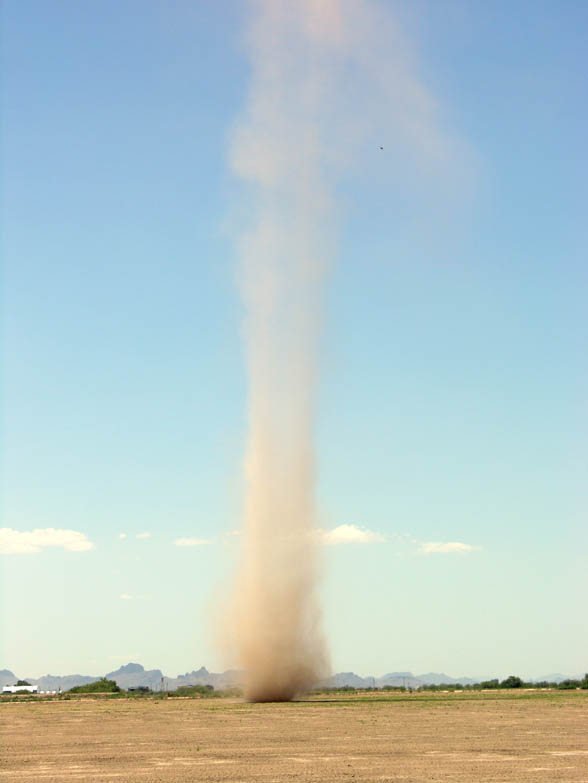
\includegraphics[width=0.6\linewidth]{Dust_devil}
      \end{center}
      \begin{center}
        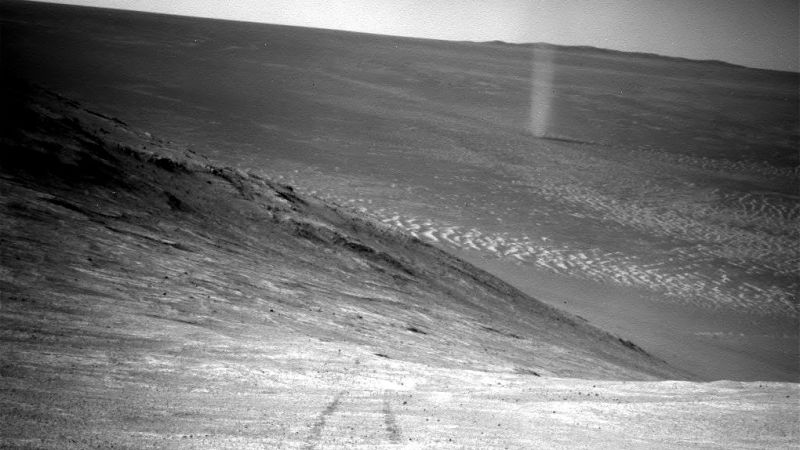
\includegraphics[width=0.8\linewidth]{martian_dust}
      \end{center}
    \end{column}
  %
    \begin{column}{0.55\linewidth}

      \begin{block}{Turbulent, unstable motions}
        \begin{itemize}
	 \item Incident solar energy absorbed into ground
	       \begin{itemize}
		\item peak solar insolation 1000~W/$\text{m}^2$ 
	       \end{itemize}
	 \item Ground heats air by conduction
	 \item Heated air expands, lowering density, 
	       driven upward by force of buoyancy
	 \item Arizona in Summer ($\Delta T= 30$ K) 
	 \item $\text{Ra} \approx 10^9 - 10^{11} \rarrow$ 
	       unstably stratified fluid
	 \item Velocities can exceed 33 m/s.
        \end{itemize}
      \end{block}
      How much energy is present in one of these objects? 
      \end{column}
    \end{columns}
  \end{frame}

%
%
%
\begin{frame}
\frametitle{Energy Estimate [Sinclair, Battan, etc. ]}

   \begin{center}
    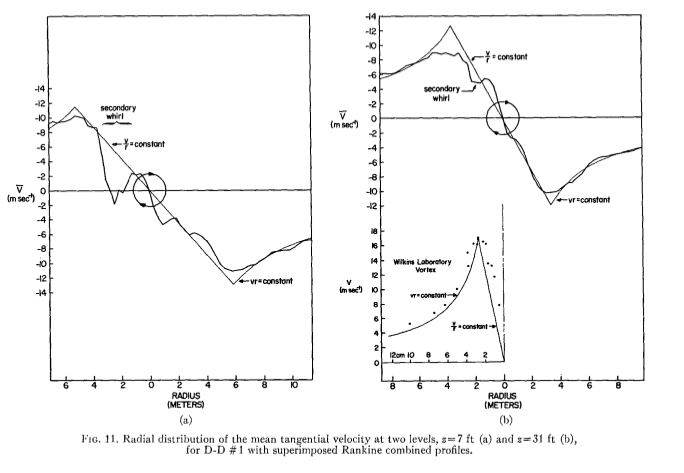
\includegraphics[width=0.6\linewidth]{sinclair_cut}
   \end{center}

\begin{itemize}
  \item Estimate energy from Sinclair's measured velocities 
  \item R $\approx$ 5 meters, $V_{\theta} \approx V_{z} \approx 10$ m/s 
  \item Kinetic Energy flux $ = \frac{1}{2}\rho \int V_z (V_z^2 + V_{\theta}^2)
	\, dA \approx 45$ kW
 \begin{itemize}
  \item Exceeds PV per $\text{m}^2$
 \end{itemize}
\end{itemize}

\end{frame}

\begin{frame}
\frametitle{Dust Devil Structure [Sinclair,Kanak,Renno]}

\begin{columns}[]
  \begin{column}{0.45\linewidth}
   \begin{center}
    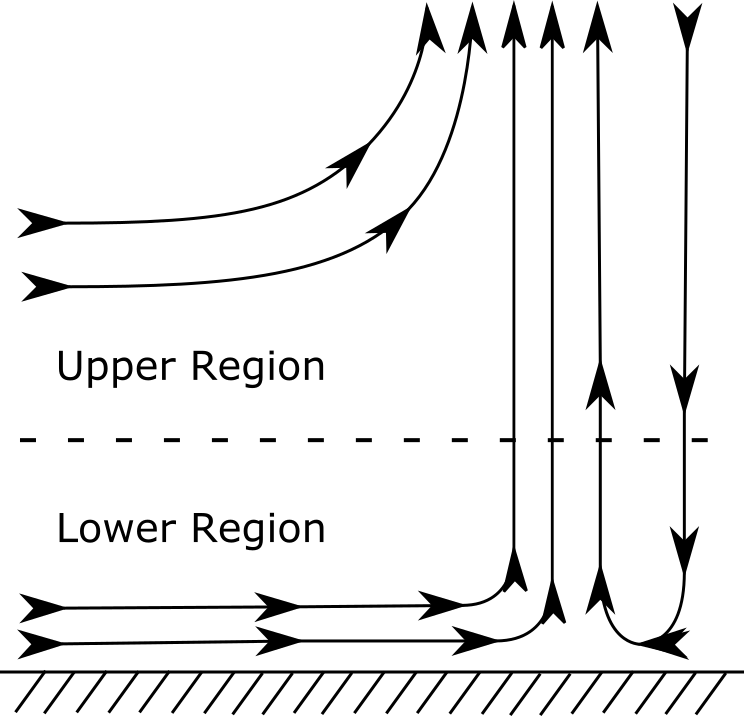
\includegraphics[width=0.9\linewidth]{ground}
   \end{center}
  \end{column}
  %
  \begin{column}{0.55\linewidth}
    \begin{block}{Dust devil structure}
    \begin{itemize}
     \item Driven by buoyancy of hot ground
     \item Near surface: radial inflow spinning region (core) 
     \item Downward flow in \myred{hot}, low-pressure  center (``eye'')
     \item Fluid from higher region entrained (inviscid potential flow region)
     \item Characterized by strong rotation
     \begin{itemize}
      \item What generates vorticity?
        \begin{itemize}
        \item vortex stretching
        \item vortex tilting
          \end{itemize}
     \end{itemize}
    \end{itemize}
   \end{block}
  \end{column}
\end{columns}

\end{frame}


%
%
%
\begin{frame}
\frametitle{Synthetic Dust Devils}

\begin{columns}[]
  \begin{column}{0.45\linewidth}
   \begin{center}
    \includegraphics[width=0.9\linewidth]{ground_vanes}
   \end{center}
  \end{column}
  %
  \begin{column}{0.55\linewidth}
   \begin{block}{Motivation}
    \begin{itemize}
     \item Engineer synthetic vortices for energy generation
       \begin{itemize}
	\item Two tier configuration mimics natural phenomenon
	\item Turbine at upper tier vanes to extract energy
       \end{itemize}

     \item Difficult to explore space experimentally
	   \begin{itemize}
	    \item Field tests in Arizona (GT)
	    \item expensive to alter configuration
	    \item difficult to measure everything
	   \end{itemize}
    \end{itemize}
   \end{block}

  \end{column}
\end{columns}
   
\end{frame}

%
%
%
\begin{frame}
\frametitle{Example configuration}

\begin{columns}[]
  \begin{column}{0.5\linewidth}

   \begin{center}
    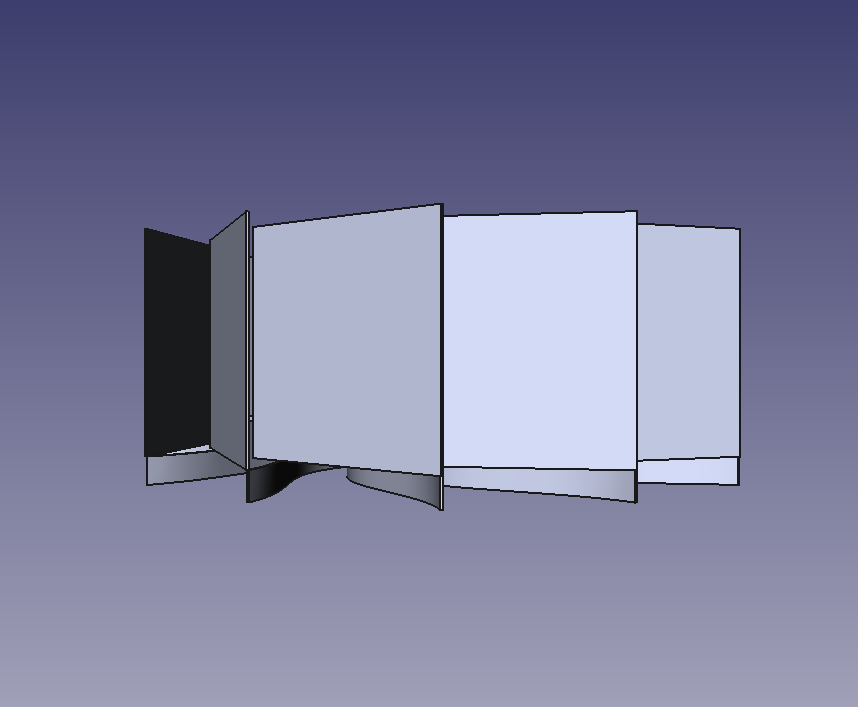
\includegraphics[width=0.8\linewidth]{side_example}
   \end{center}


  \end{column}
  %
  \begin{column}{0.5\linewidth}

   \begin{center}
    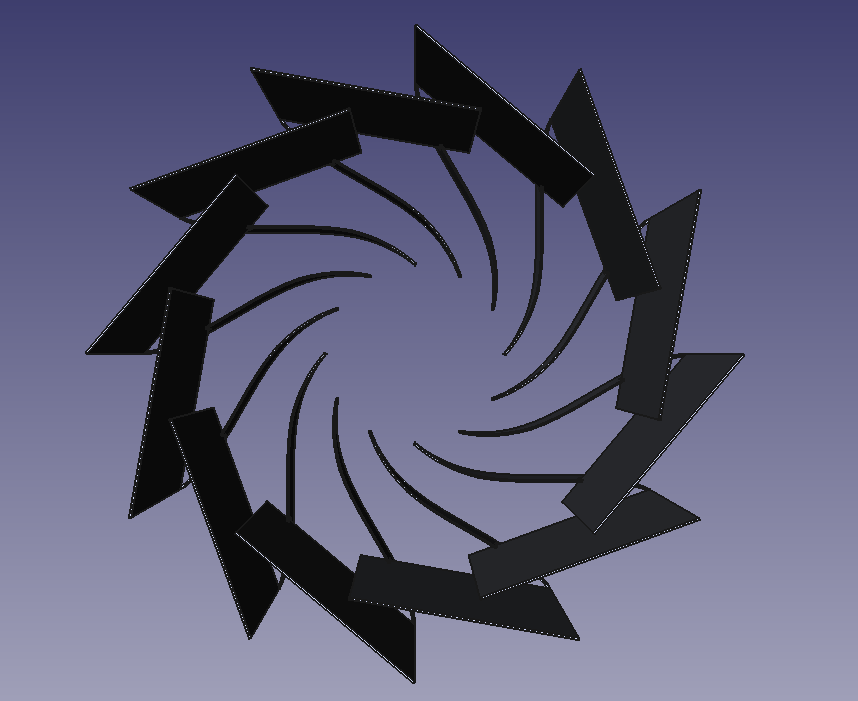
\includegraphics[width=0.8\linewidth]{top_example}
   \end{center}

  \end{column}
\end{columns}

   \begin{block}{Turning Vanes}
    \begin{itemize}
     \item Several control surfaces used to turn the flow
     \item Top tier significantly taller than the bottom
     \item A cone may be added to the top to contract the flow
     \item A turbine is placed above the vanes to extract kinetic energy
    \end{itemize}
   \end{block}
   
\end{frame}



%
%
%
\begin{frame}
\frametitle{Project Objectives}

 \begin{block}{System Feasibility Assessment}
  \begin{itemize}
   \item Assess technological capability
  \end{itemize}
 \end{block}


 \begin{block}{Scenario Space}
  \begin{itemize}
   \item Atmosphere, buoyancy, winds, etc. 
  \end{itemize}
  \end{block}

 \begin{block}{Solar Vortex (SoV) System Configuration}
 \begin{itemize}
  \item Represent complex configuration with CFD
	\begin{itemize}
	 \item Turning vanes
	 \item Cone (and solid surfaces)
	 \item Turbine
	\end{itemize}
  \item Inform design for 2016 field test
	\begin{itemize}
	 \item Probe and optimize SoV configuration
	 \item Predict energy output
	\end{itemize}
 \end{itemize}
 \end{block}

\end{frame}


%===============================================================================

\section{Modeling}
%
%


%
%
%
\begin{frame}
\frametitle{Dynamical Equations}
The equations describing fluid flow with natural convection are,
\begin{align}
  \frac{\partial {\bf u}}{\partial t} + {\bf u} \cdot \nabla {\bf u} =& \,
  -\frac{1}{\rho}\nabla P + \nu \nabla^2 {\bf u} \textcolor{orange}{-
 {\bf g} \frac{T-T_0}{T_0}}\\
  \nabla \cdot {\bf u} =& \, 0 \\
  \rho c_p \frac{\partial T}{\partial t} + {\bf u} \cdot \nabla T =& \, \nabla
 \cdot ( K \nabla T)
\end{align} 

\begin{itemize}
  \item Incompressible N-S + \textcolor{orange}{Boussinesq buoyancy}
  \item Temperature variation small compared to mean temperature
  \item Low mach number
\end{itemize}
\begin{center}
  However, $Ra \approx 10^9 - 10^{11}$ -- \textcolor{blue}{Need turbulence model!}
\end{center}
\end{frame}

%
%
%
\begin{frame}
\frametitle{Diffusivity Modeling}
 
 \begin{columns}[]
  \begin{column}{0.45\linewidth}

 MO (spatially homogeneous)

  \end{column}
  \begin{column}{0.55\linewidth}

   \begin{center}
    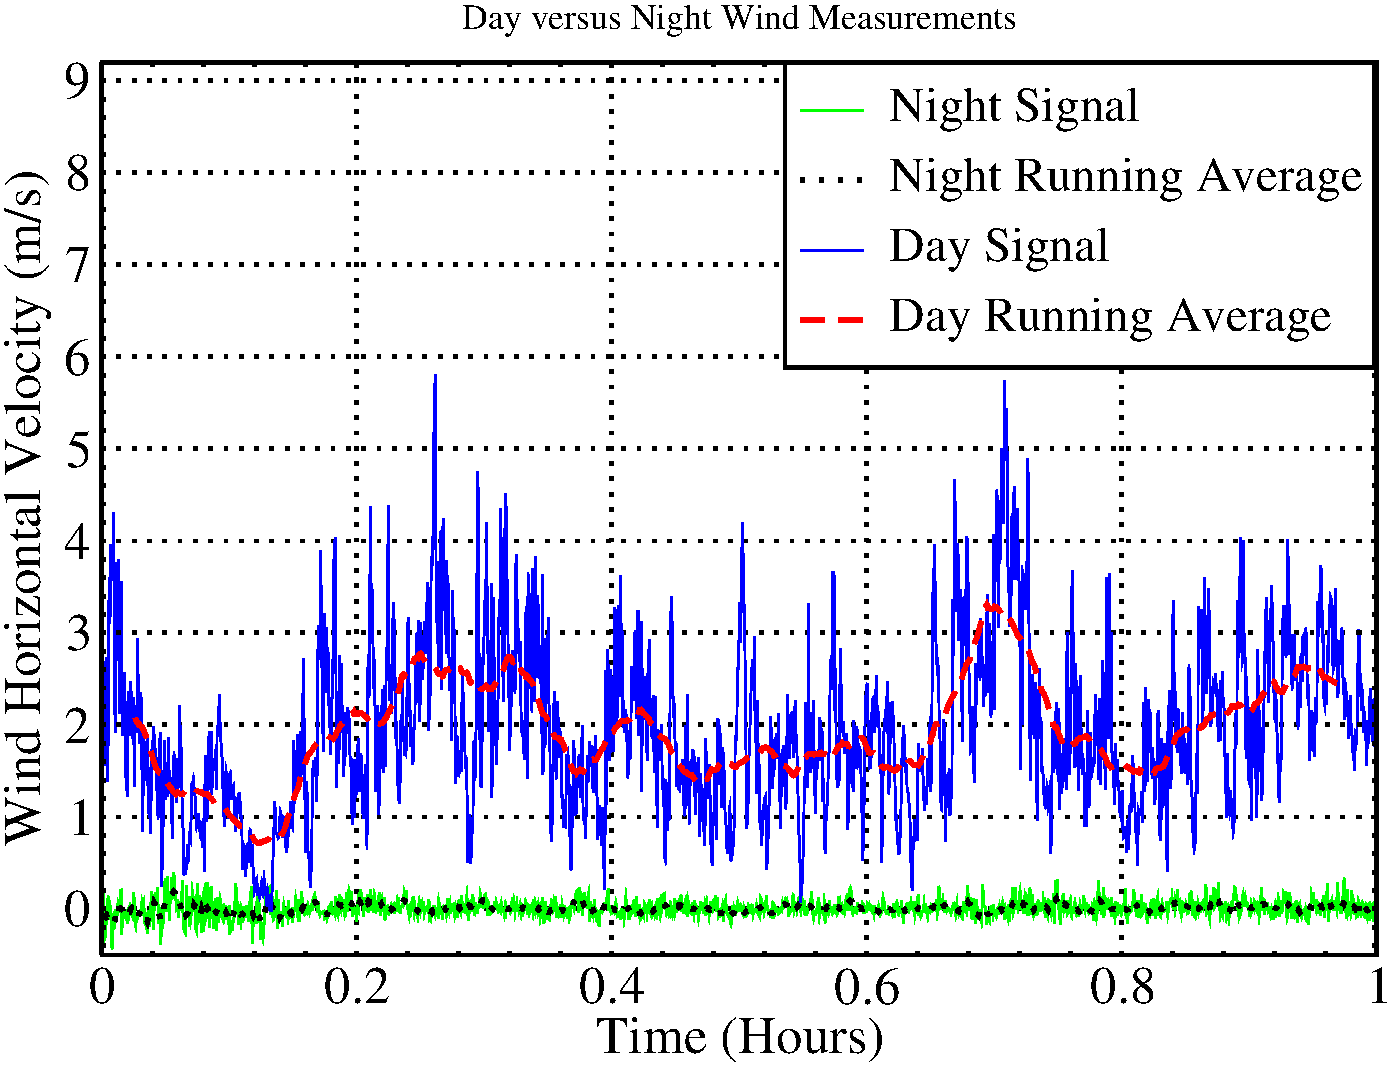
\includegraphics[width=0.8\linewidth]{wind_measurements}
   \end{center}
   
  \end{column}
\end{columns}

\end{frame}

%
%
%
\begin{frame}
\frametitle{Scenario Modeling}
 
 \begin{columns}[]
  \begin{column}{0.45\linewidth}

 winds

 thermal

  \end{column}
  \begin{column}{0.55\linewidth}

   \begin{center}
    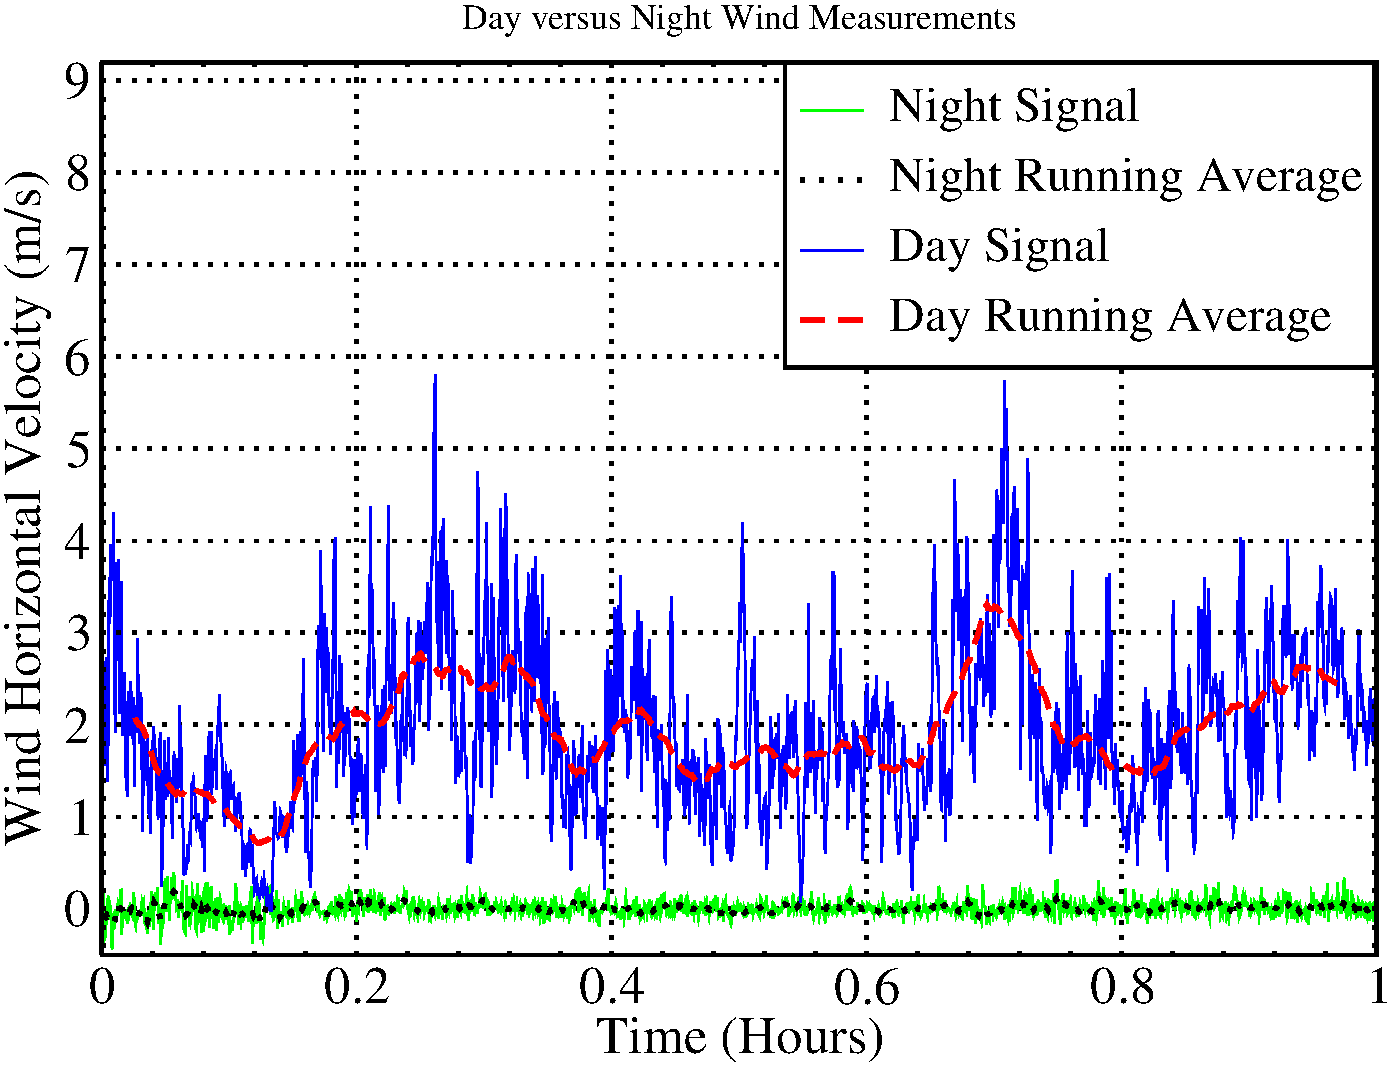
\includegraphics[width=0.8\linewidth]{wind_measurements}
   \end{center}
   
  \end{column}
\end{columns}

\end{frame}


%
%
%
\begin{frame}
\frametitle{Turning Vane Representation}

\begin{columns}[]
  \begin{column}{0.5\linewidth}

   \begin{center}
    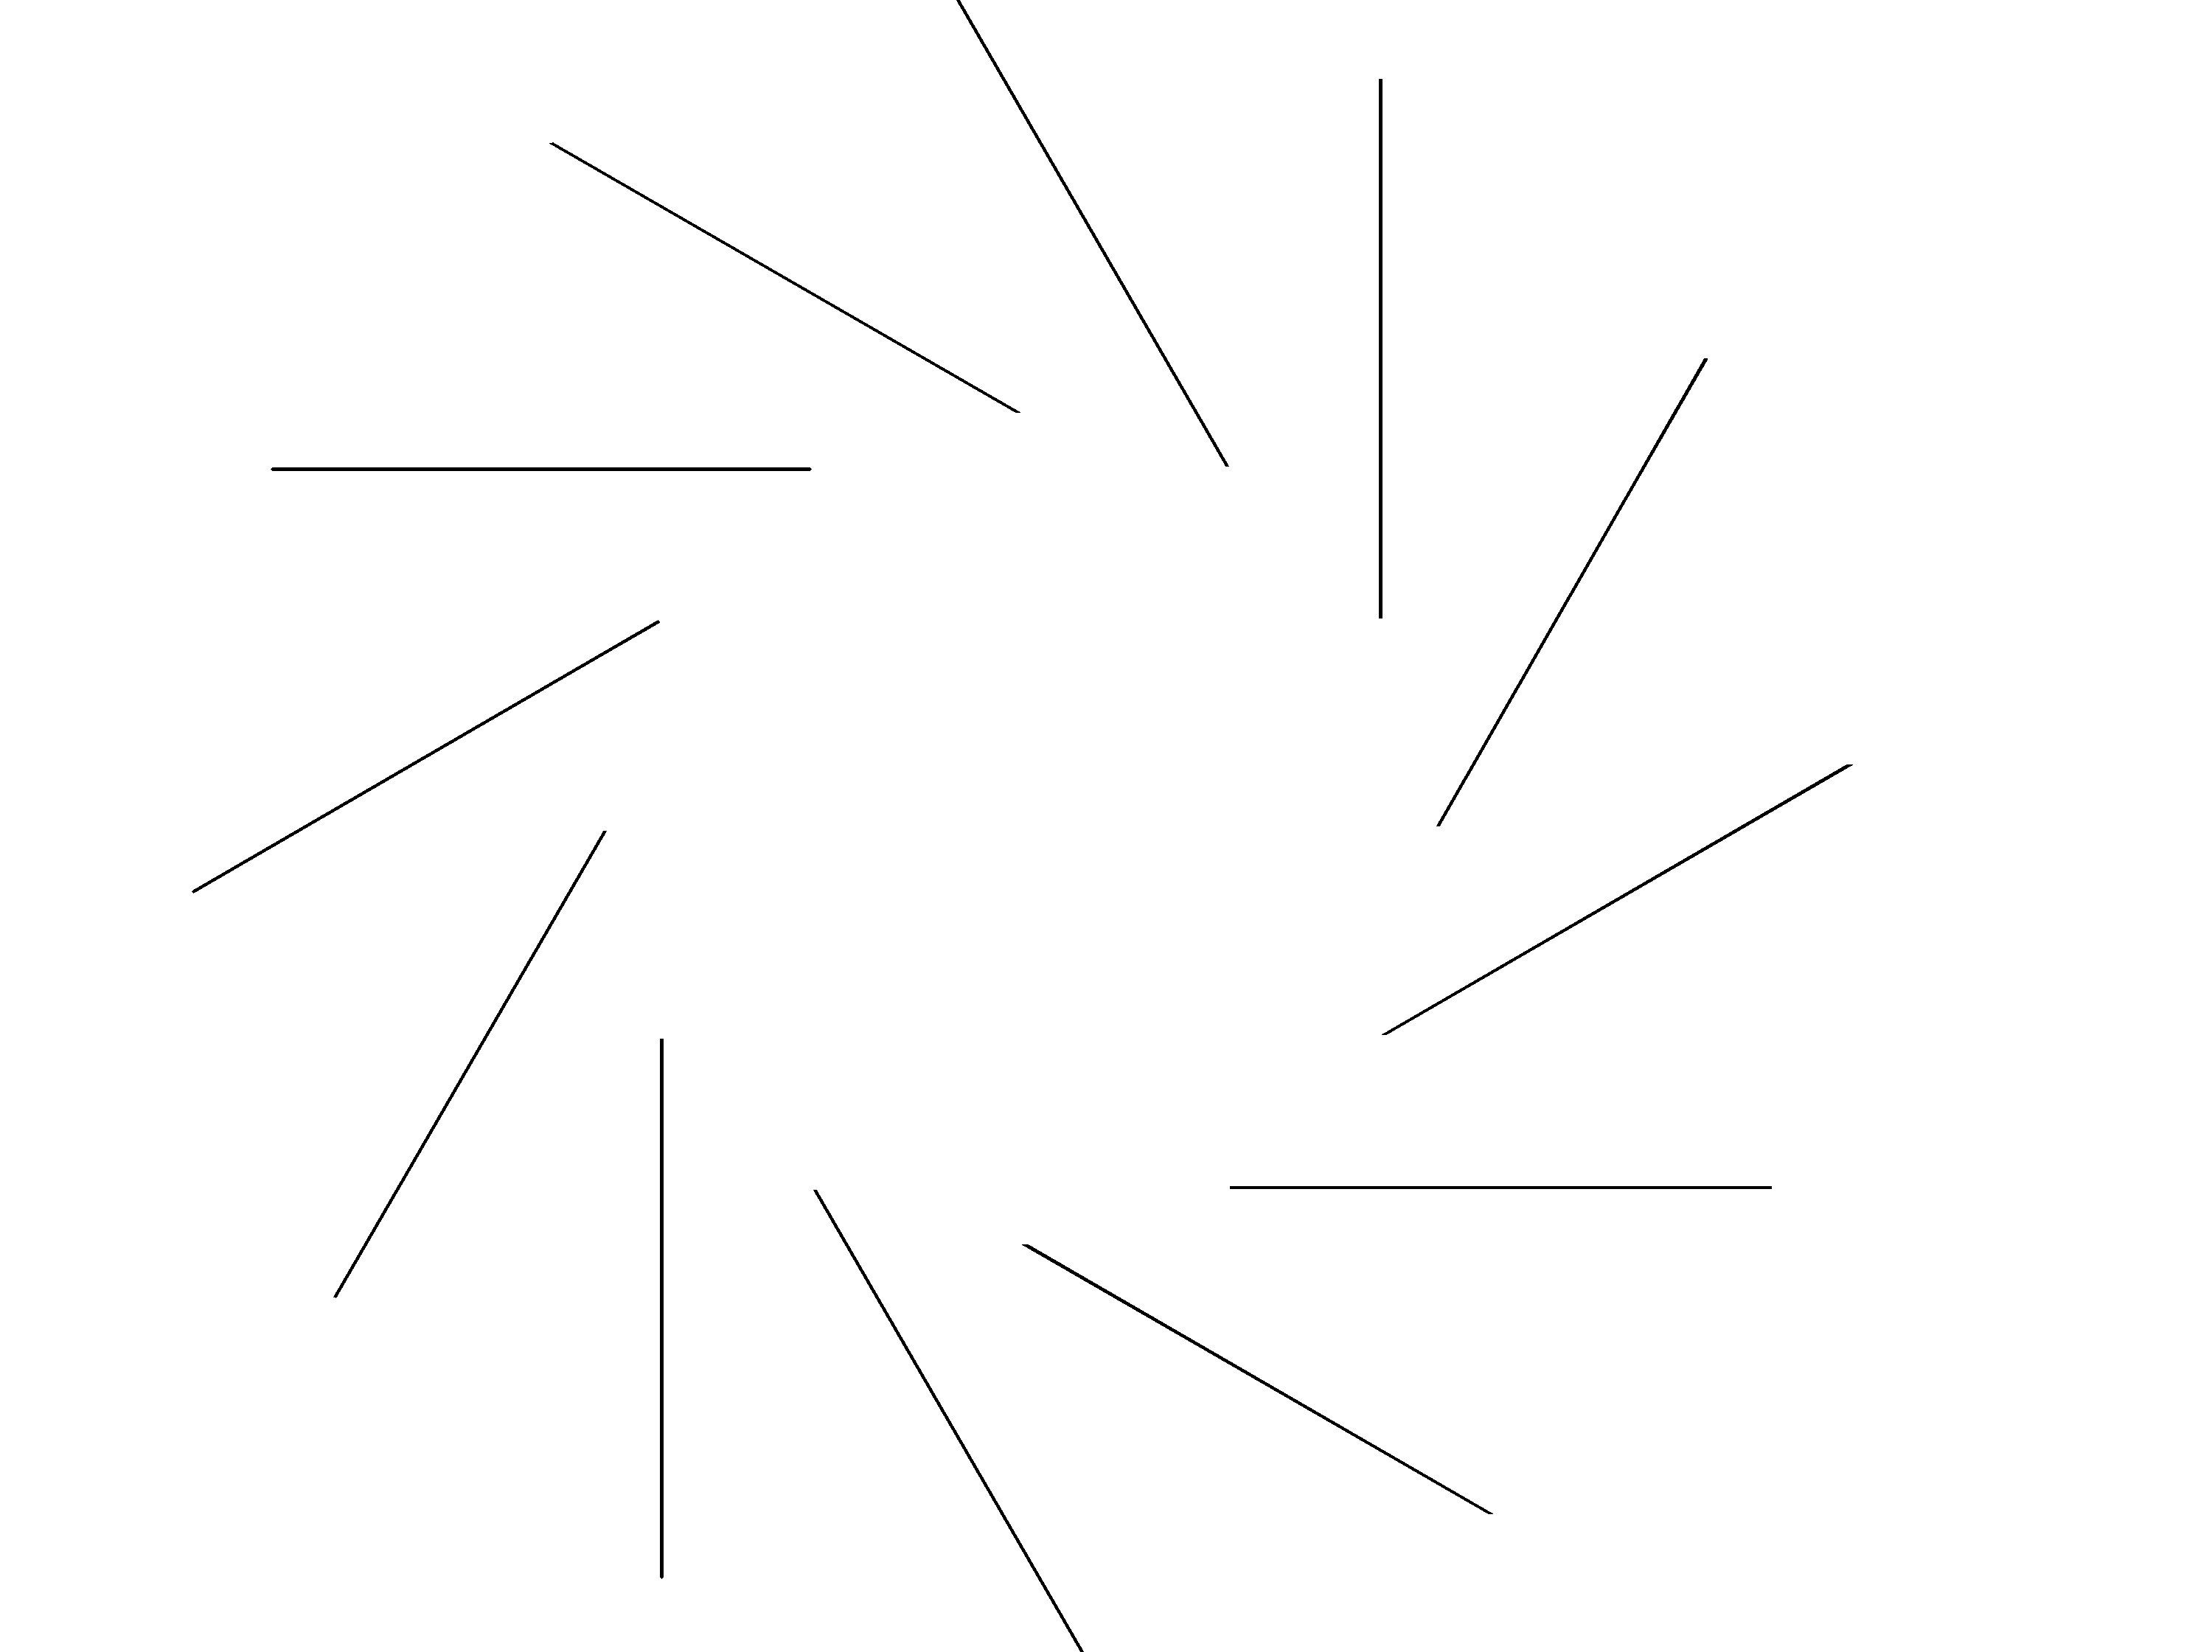
\includegraphics[width=0.65\linewidth]{gridded_region}
   \end{center}

  \end{column}

  \begin{column}{0.5\linewidth}
   \begin{center}
    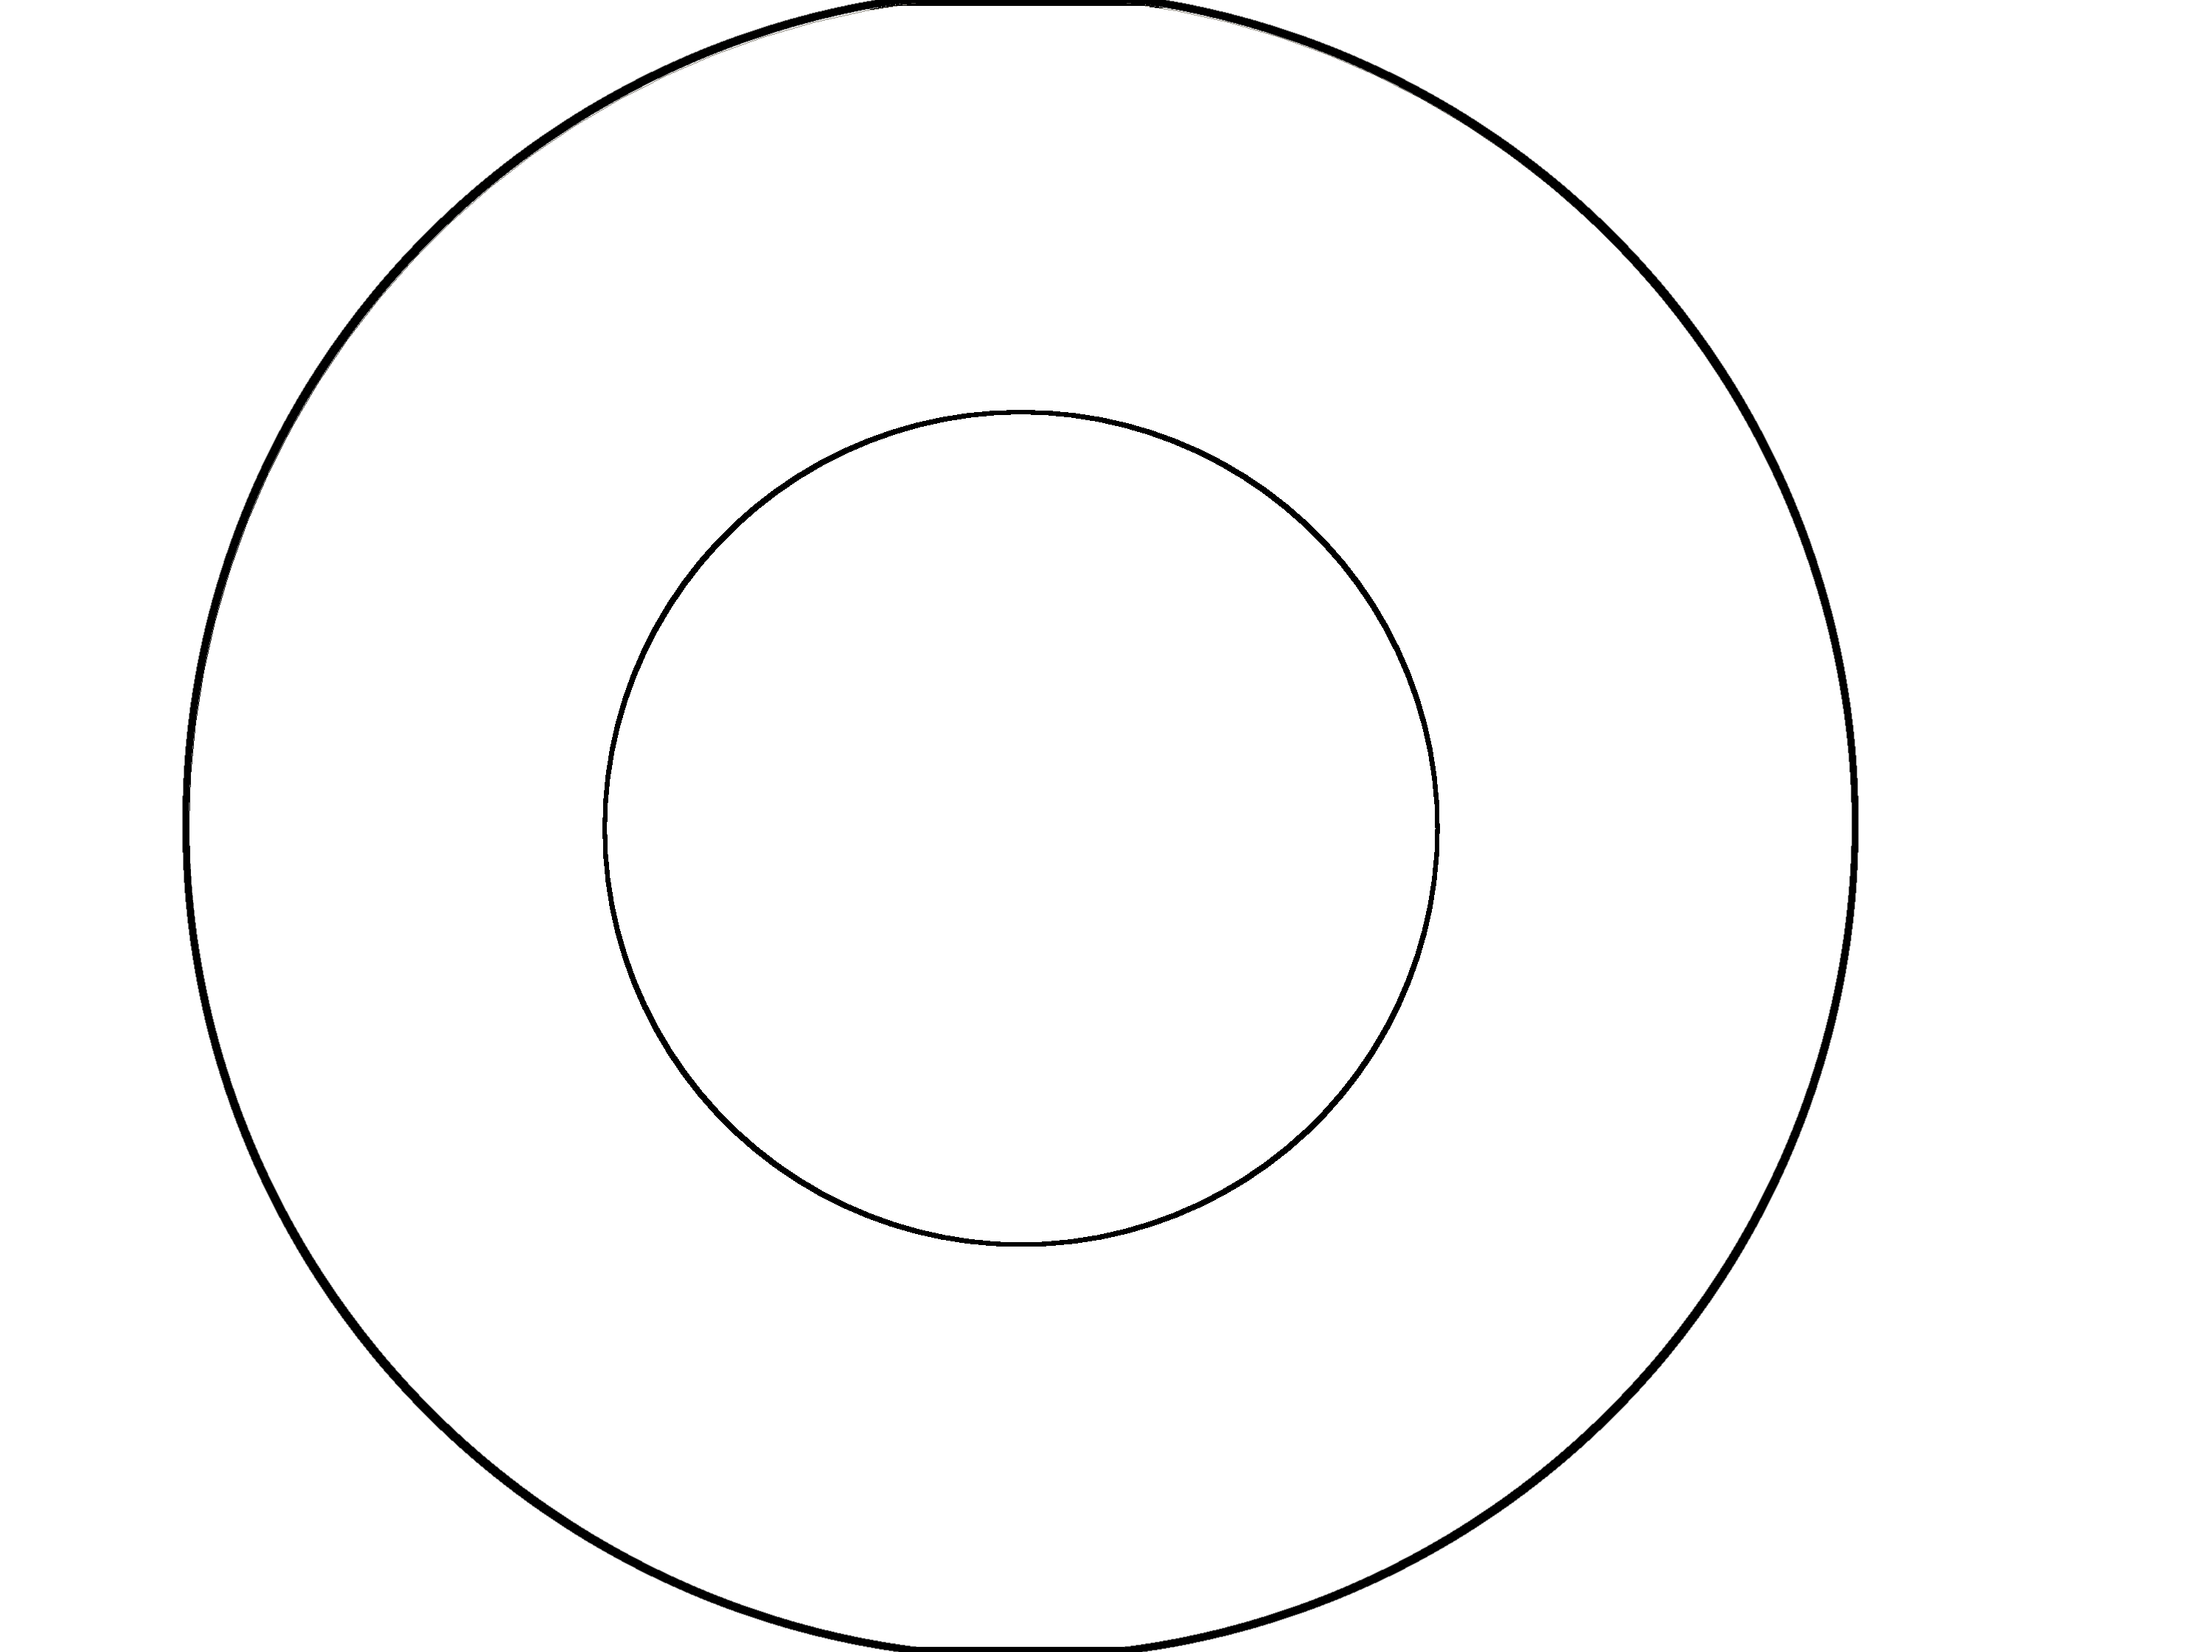
\includegraphics[width=0.5\linewidth]{forcing_region}
   \end{center}

  \end{column}
\end{columns}


 \begin{block}{Virtual Vanes}

  \begin{itemize}
   \item Volumetric forcing: 
	 \begin{itemize}
	  \item Very general formulation, no re-meshing 
	  \item Vane surface not represented
	  \item Similar to actuator-disk
	 \end{itemize}	 
%  \end{itemize}
%  
%  \begin{itemize}
%   \item Unit normal to vane surface, 
%	 \begin{equation}
%	  {\bf n}({\bf x}) = \sin \left(\textcolor{red}{\phi(r)} \right) \hat{{\bf r}}+ \cos
%	   \left(\textcolor{red}{\phi(r)} \right) \hat{{\bf \theta}} 
%	 \end{equation}
   \item Apply ${\bf f_v}$ to force flow parallel to vanes,
	 \begin{equation}
	  {\bf f}_v= -\frac{1}{\textcolor{red}{\ell_v}}|{\bf u}|({\bf u}\cdot{\bf n_v}){\bf n_v}
	 \end{equation}
  \end{itemize}
 \end{block}

\end{frame}

%
%
%
\begin{frame}
\frametitle{Wind Cases}

\begin{block}

   \begin{center}
    \includegraphics[width=0.7\linewidth]{wind_3d}
   \end{center}

   \begin{itemize}
   \item Specified Inflow (Dirichlet)
   \item Top and Outflow have special mixed B.C.
   \item Sponge layers on Top and Outflow
   \item Natural (do nothing) boundaries on the side (Neumann)
   \end{itemize}

\end{block}
\end{frame}


%
%
%
\begin{frame}
  \frametitle{Numerics}
  \begin{block}{Formulation}
    \begin{itemize}
    \item Using Galerkin FEM discretization (N-S in weak form)
    \item Stabilized with SUPG stabilization \textit{al la} Hughes/Becker+Braack
      \begin{itemize}
      \item Adjoint stabilization scheme ($\tau$)
      \end{itemize}
    \item Time discretization via backward Euler \textcolor{blue}{(if not steady)}
    \item Newton method used to solve resulting non-linear implicit system
    \end{itemize}
  \end{block}

  \begin{block}{Software}
    \begin{itemize}
    \item Using GRINS(+Libmesh) library developed by Bauman and Stogner
    \end{itemize}
  \end{block}

  \begin{block}{Hardware}
    \begin{itemize}
    \item Runs performed on LS4,LS5, Stampede at TACC
    \item 264-528 processing cores
    \item Several million degrees of freedom for each run, locally $O(10^4)$ 
    \end{itemize}
  \end{block}

\end{frame}


%
%
%
\begin{frame}
  \frametitle{Modeling Hierarchy}

    \begin{center}
    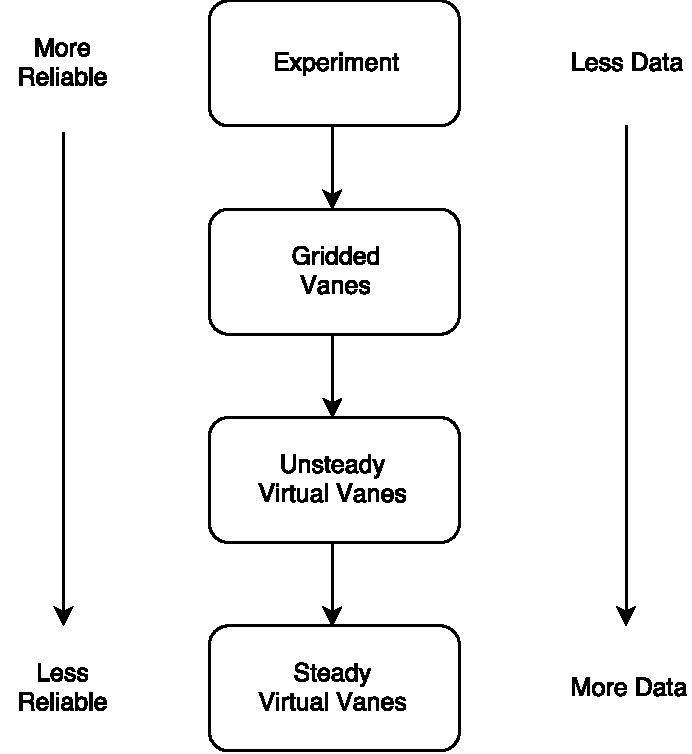
\includegraphics[width=0.5\linewidth]{validation_hierarchy}
   \end{center}

\end{frame}

%
%
%
\begin{frame}
 \frametitle{Validation}

 \begin{columns}[]
  \begin{column}{0.55\linewidth}

   \begin{block}{Scenarios and Configurations}
    \begin{itemize}
     \item Tabletop Laboratory
     \item Cold Wind Tunnel
     \item Field Tests
     \item Hierarchy of CFD models 
	   \begin{itemize}
	    \item Gridded vs. virtual
	    \item Steady vs. unsteady
	    \item Sensitivities to QoI
	   \end{itemize}
    \end{itemize}
    \end{block}

  \end{column}

  \begin{column}{0.45\linewidth}
  \begin{center}
   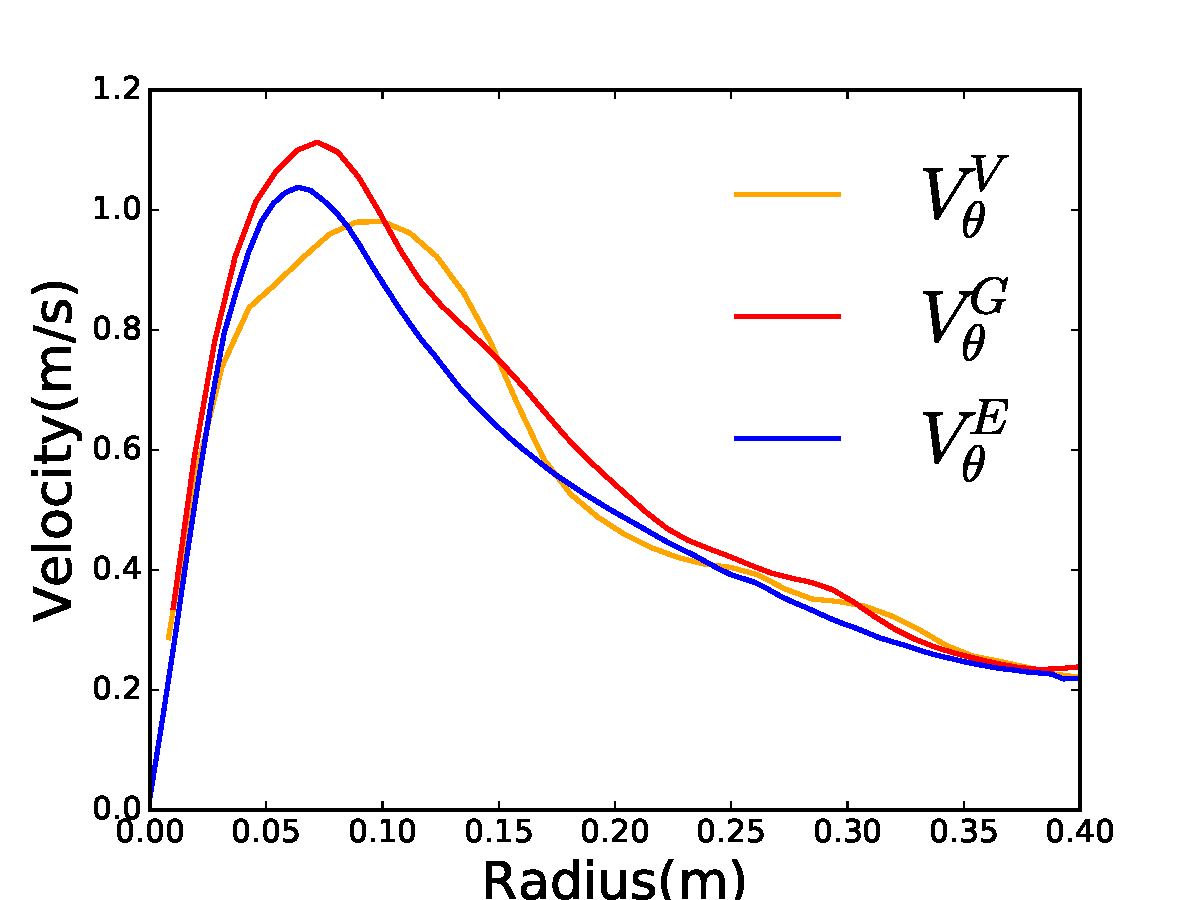
\includegraphics[width=.85\linewidth]{sim_vs_exp_30_vt}
  \end{center}
  \end{column}
  \end{columns}

 %
 % 2nd column
 
 \begin{columns}[]
  \begin{column}{0.55\linewidth}
   
   \begin{center}
    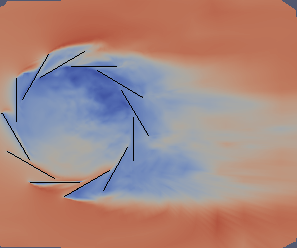
\includegraphics[width=.55\linewidth]{gridded_wind}
   \end{center}
\end{column}
 \begin{column}{0.55\linewidth}
   \begin{center}
    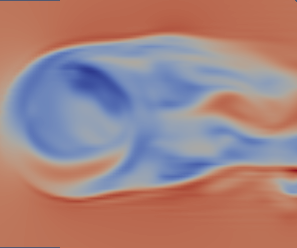
\includegraphics[width=.55\linewidth]{virtual_wind}
   \end{center}
\end{column}
 \end{columns}


\end{frame}


%===============================================================================

\section{Optimization Heuristics}
%
%
\begin{frame}
 \frametitle{Optimization}

    \begin{figure}[htb]
     \centering
     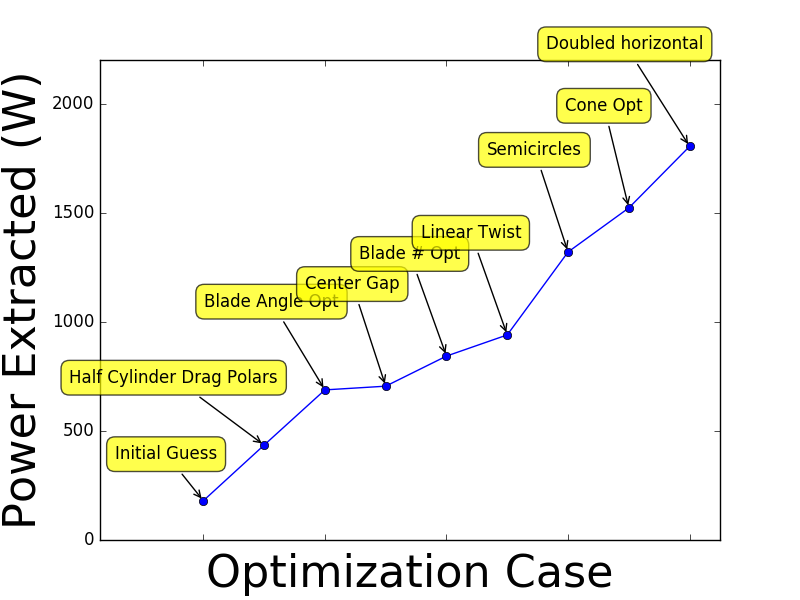
\includegraphics[width=.53\linewidth]{turbine_opt}
    \end{figure}
 


\end{frame}


%===============================================================================

\section{2016 Field Test}
%
%

%\begin{columns}
%  \begin{column}{0.5\linewidth}

\begin{frame}
 \frametitle{Top Tier Vanes}
    \begin{figure}[htb]
     \centering
     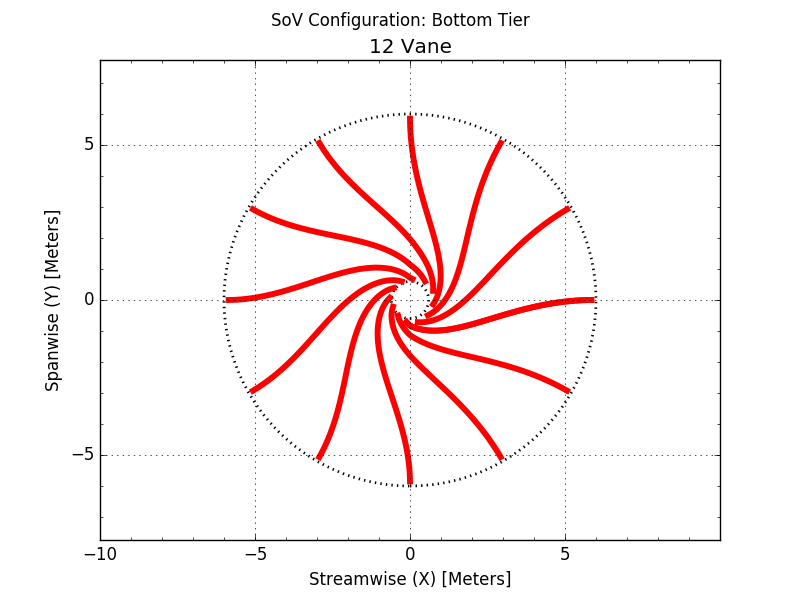
\includegraphics[width=.53\linewidth]{interp_entire_top}
    \end{figure}

%   \end{column}

%   \begin{column}{0.5\linewidth}
%    \begin{tabular}{l|l|l}
%     Name                        & Value & Meaning                    \\
%     \hline
%     $r^{\text{cyl}}$            &  3.0 meters & Radius of rigid cylinder
% 	    \\ 
%     $r^t_{\text{min}}$          &  3.0 meters & Smallest radius of top
% 	    tier vanes, relative to ground \\ 
%     $L_x$                       &  12 meters  & Distance upstream
% 	    of vanes relative to center\\
%     $\phi^{t,l}$ &  $0^{\circ}$   & Outer angle for the top tier, left
% 	    side vanes \\ 
%     $\phi^{t,r}$   &  $0^{\circ}$   & Outer angle for the top tier right
% 	    side \\ 
%     $\theta^{t,l}$ &   $30^{\circ} +\frac{\alpha}{3}$  & Inner angle for
% 	    the top tier left side vanes\\ 
%     $\theta^{t,r}$   &   $75^{\circ} +\frac{\alpha}{6}$   & Inner angle
% 	    for the top tier right side \\ 
%     $L^{t,r}$                   &  12 meters  & Width of vane in front of
% 	    cylinder \\ 
%     $L^{t,l}$                   &  10 meters  & Width of vane to the side
% 	    of cylinder \\ 
%    \end{tabular}
   
% yar  
%   \end{column}
% \end{columns}
 
 \begin{block}{}
  \begin{itemize}
   \item Vanes aligned with streamwise (wind) velocity
   \item Vanes contract flow into central region
   \item Impermeable half cylinder arc
   \item 6 meter inner diameter
  \end{itemize}
 \end{block}
\end{frame}

%
%
%
\begin{frame}
 \frametitle{Effect of the Wind}

 connection between synthetic and natural is tenuous at best but this is
 an interesting implication for impact of wind in real phenomenon
 
 \begin{figure}[htb]
  \centering
  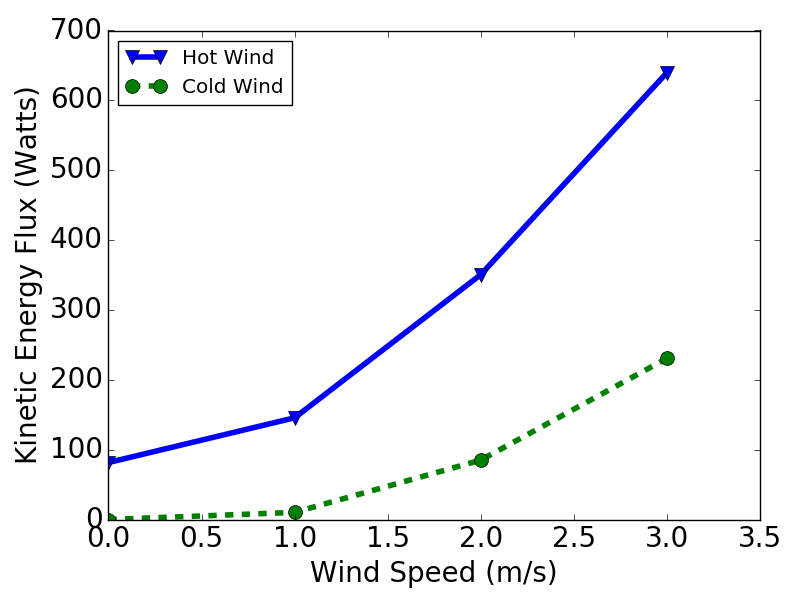
\includegraphics[width=.55\linewidth]{wind_impact}
 \end{figure}
 
\end{frame}

%
%
%
\begin{frame}
 \frametitle{Bottom Tier Vanes}
    \begin{figure}[htb]
     \centering
     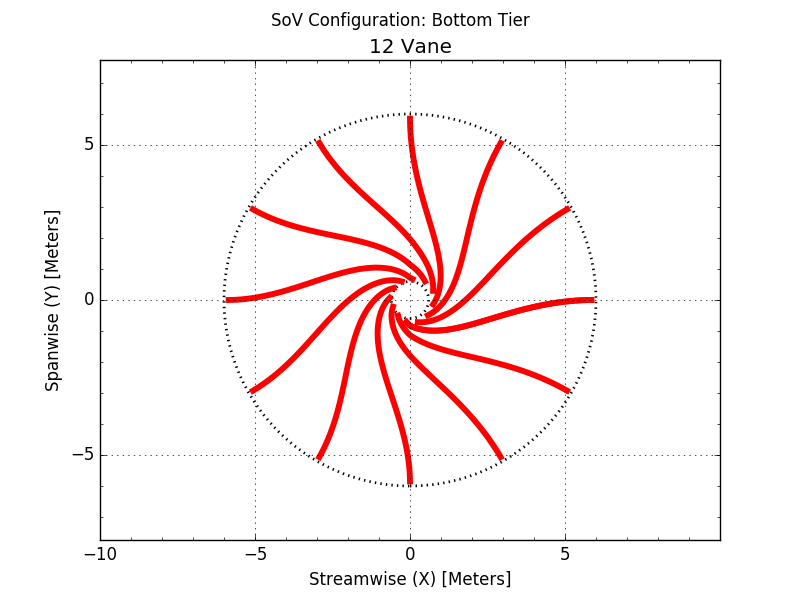
\includegraphics[width=.55\linewidth]{interp_entire_bottom}
    \end{figure}
 
 \begin{block}{}
  \begin{itemize}
   \item Bottom tier vanes not symmetric along upstream/downstream
	 sides:
	 \begin{itemize}
	  \item Different heights
	  \item Different final angles
	 \end{itemize}
   \item Significant inflow from downstream
  \end{itemize}
 \end{block}
\end{frame}

%
%
%
\begin{frame}
 \frametitle{Vertical View}
    \begin{figure}[htb]
     \centering
     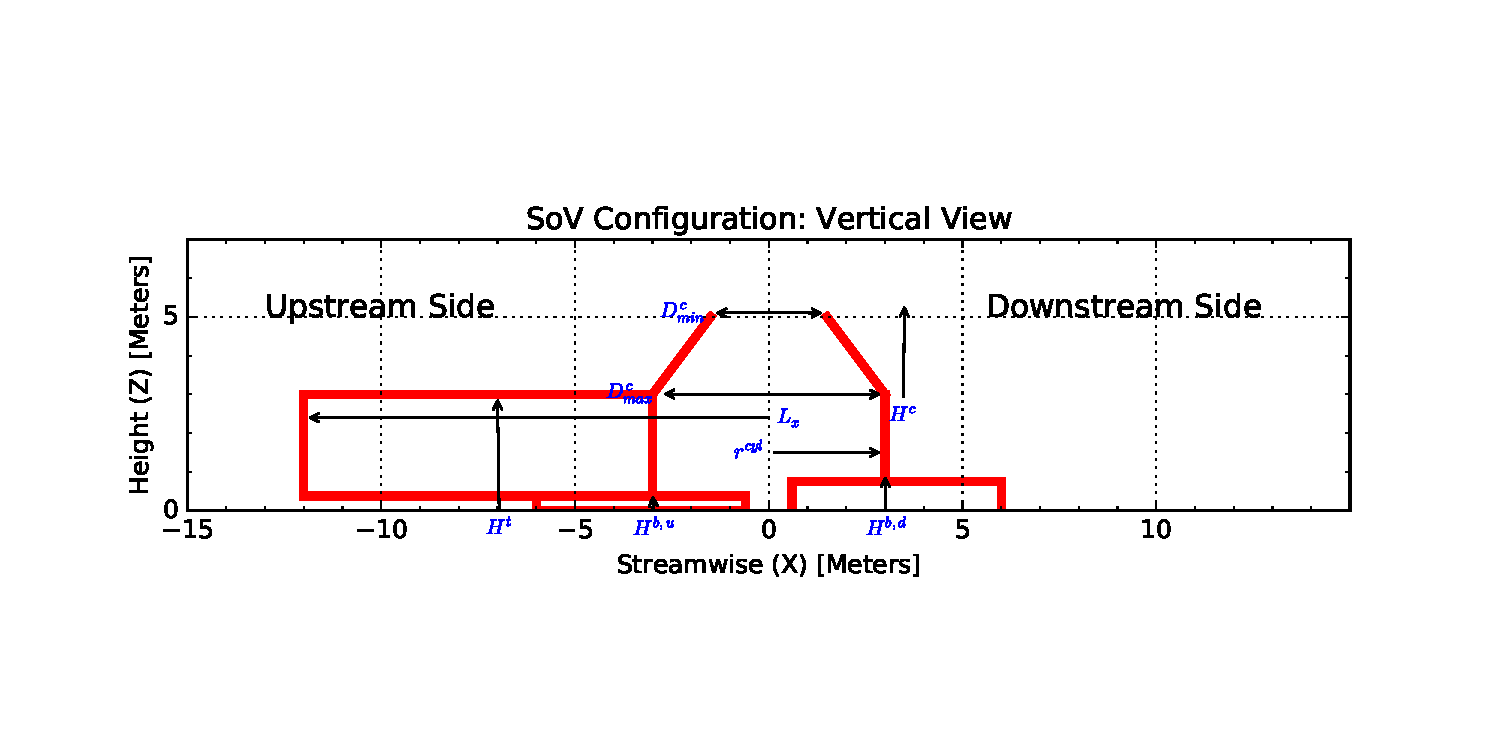
\includegraphics[width=.8\linewidth]{vertical_design}
    \end{figure}
 
 \begin{block}{}
  \begin{itemize}
   \item Cone visible
   \item Height asymmetry in bottom tier vanes visible
   \item Turbine placed at top of cone
   \item Vertical partition on top of 2nd tier vanes 
  \end{itemize}
 \end{block}
\end{frame}

%
%
%
\begin{frame}
 \frametitle{CAD drawings}

 \begin{columns}[]
  \begin{column}{0.55\linewidth}

    \begin{figure}[htb]
     \centering
     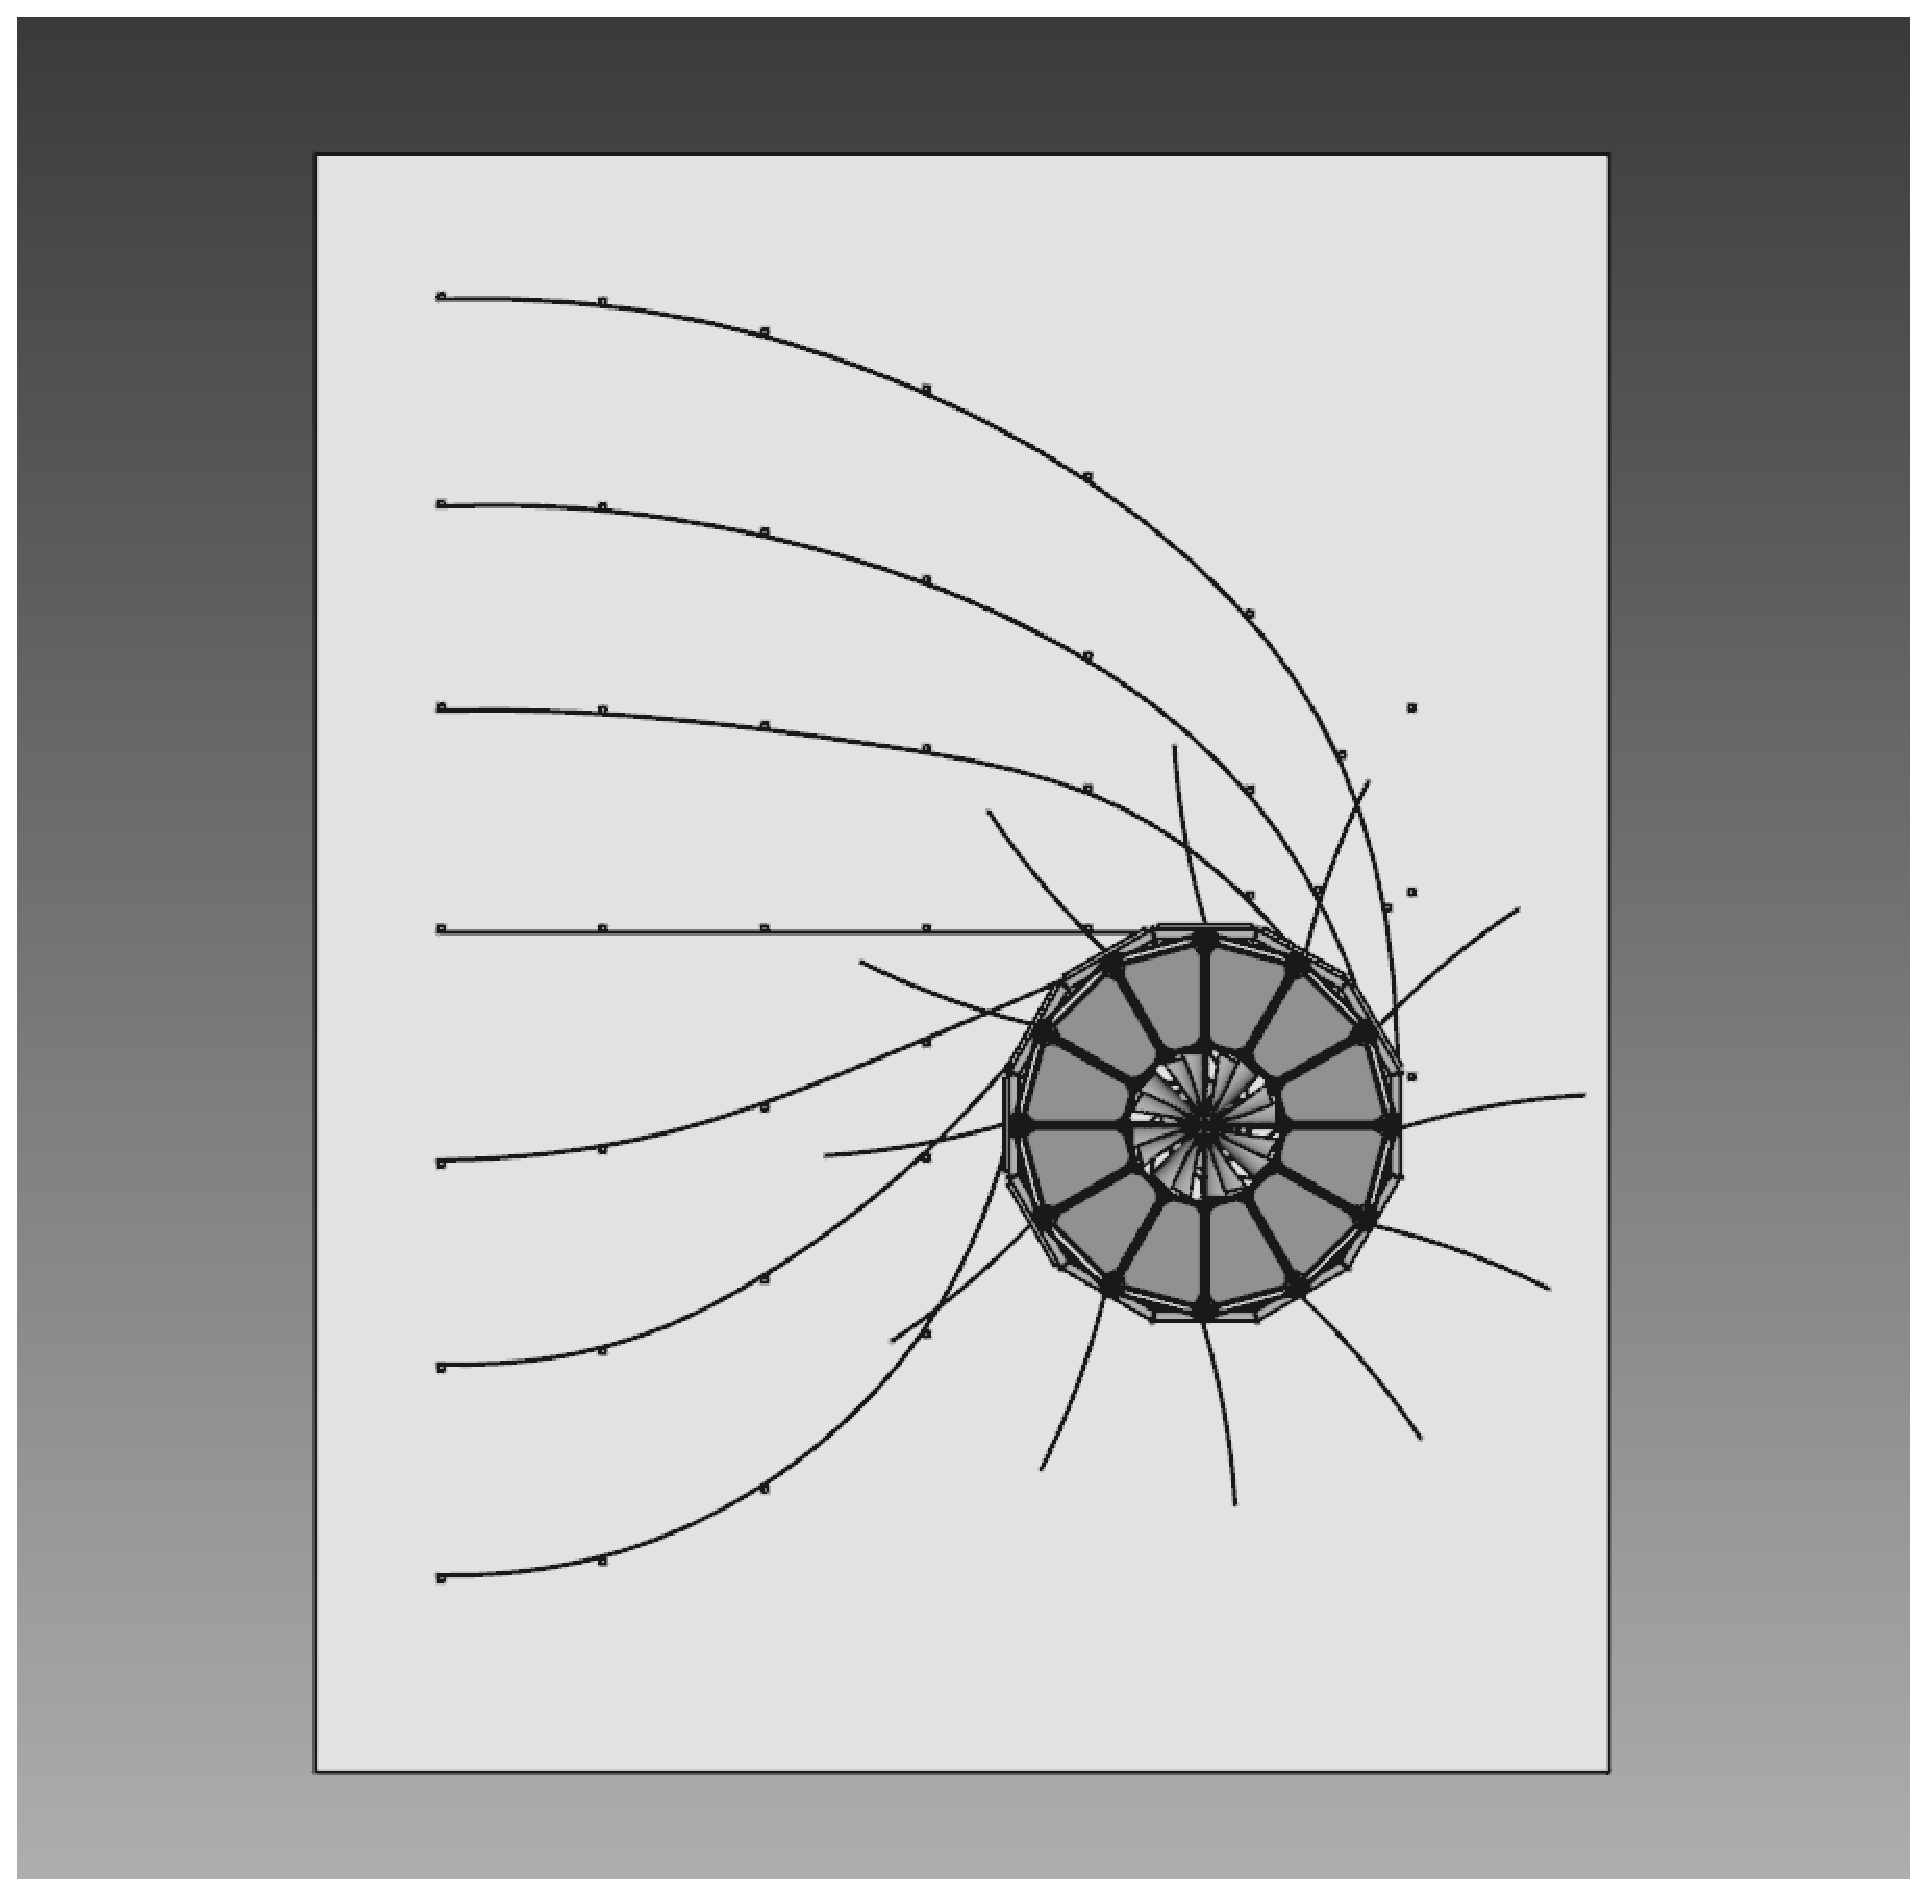
\includegraphics[width=.9\linewidth]{top_down_cad_notop}
    \end{figure}

  \end{column}
   \begin{column}{0.45\linewidth}

    \begin{figure}[htb]
     \centering
     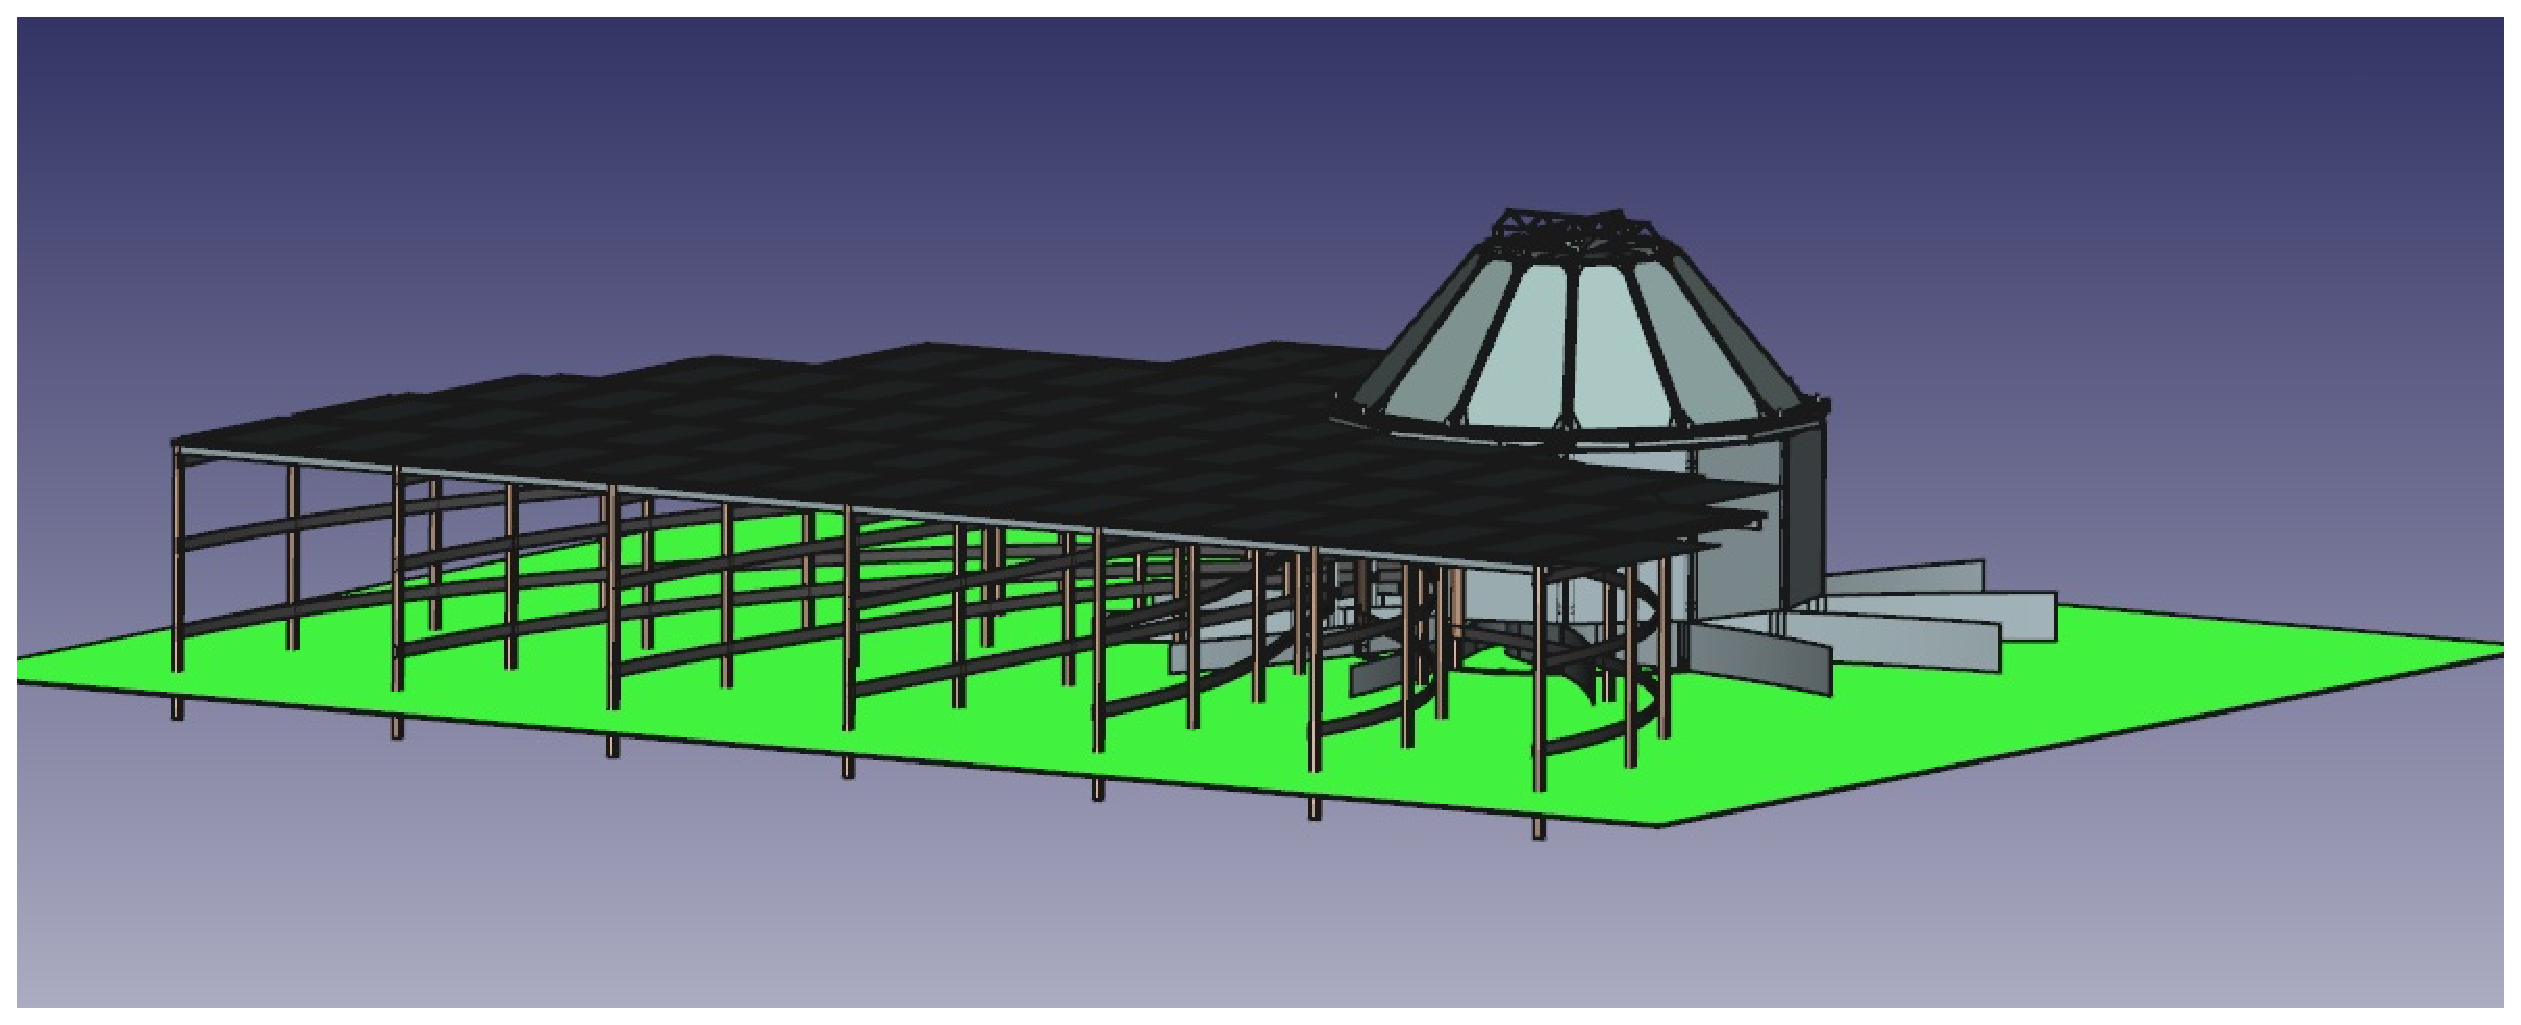
\includegraphics[width=1.0\linewidth]{skewed_cad}
    \end{figure}

    \begin{block}{Images}
     \begin{itemize}
      \item Cone clearly visible
      \item Horizontal Partitions
      \item Turning Vane Posts (drag)
      \item Consistent with field test 
      \item CAD credit: John Culp, GT
     \end{itemize}
     \end{block}

   \end{column}
 \end{columns}

\end{frame}

%
%
%
\begin{frame}
 \frametitle{Turbine Model}

 \begin{center}
  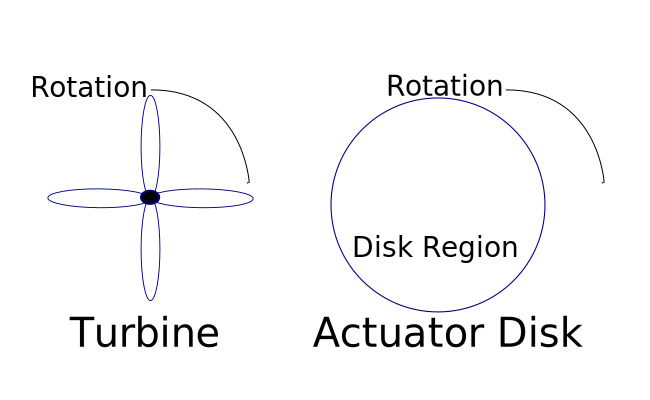
\includegraphics[width=0.58\linewidth]{actuator_disk}
 \end{center}
 
 \begin{block}{Actuator Disk (Blade Element Momentum)}
  \begin{itemize}
  \item Represents turbine blade geometry as spinning disk
  \item Assumes axisymmetric turbine, neglects unsteady effects
  \item Not validated
  \item Common in wind turbine industry
  \end{itemize}
 \end{block}

\end{frame}

%
%
%
\begin{frame}
 \frametitle{Turbine Model}

 common model
 math behind actuator disk equations ($F=?$)
 interpolate
 flat plate, 90, 180, etc.

   \begin{center}
    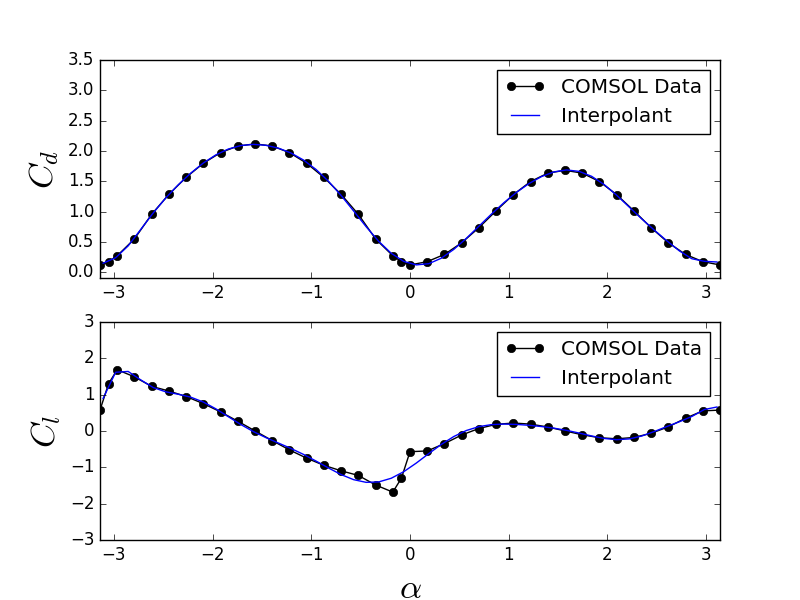
\includegraphics[width=0.5\linewidth]{90}
   \end{center}

 
\end{frame}


%
%
\begin{frame}
 \frametitle{Turbine Optimization Method}

 \begin{columns}[]
  \begin{column}{0.45\linewidth}
   \begin{center}
    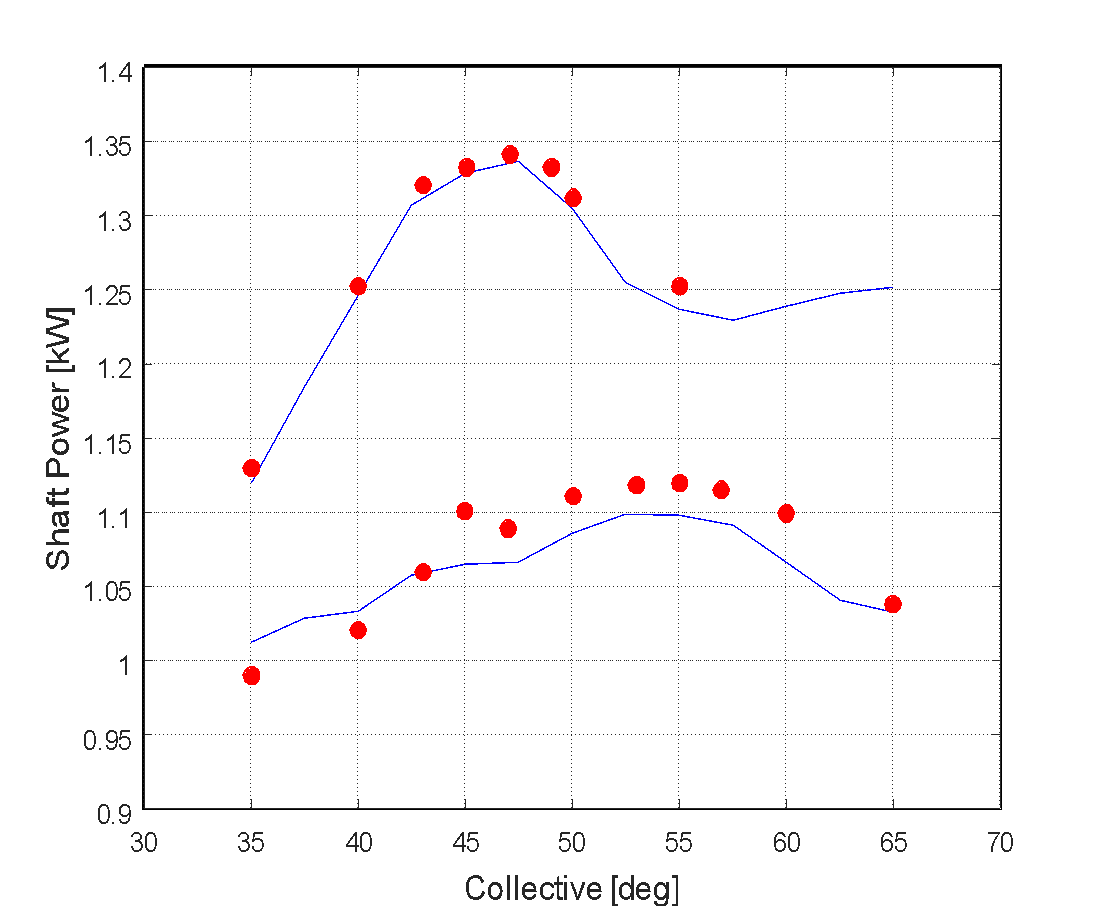
\includegraphics[width=1.05\linewidth]{utrc_plot}
   \end{center}

  \end{column}
    \begin{column}{0.55\linewidth}

     \begin{block}{Coupled Effort}
     \begin{itemize}
      \item Optimization effort based on UTRC ``frozen flow''
	    and full CFD
      \item Both use actuator disk model
      \item Frozen flow used CFD as input
      \item Iterative procedure
	    \begin{itemize}
	     \item Frozen flow prediction 
	     \item ``Validated'' by CFD
	     \item Not automated!
	    \end{itemize}
      \item Results broadly agree
	    \begin{itemize}
	     \item inflow updated after several iterations
	    \end{itemize}
     \end{itemize}

      \end{block}
    \end{column}
 \end{columns}
\end{frame}

%
%
\begin{frame}
 \frametitle{Final Design}

    \begin{figure}[htb]
     \centering
     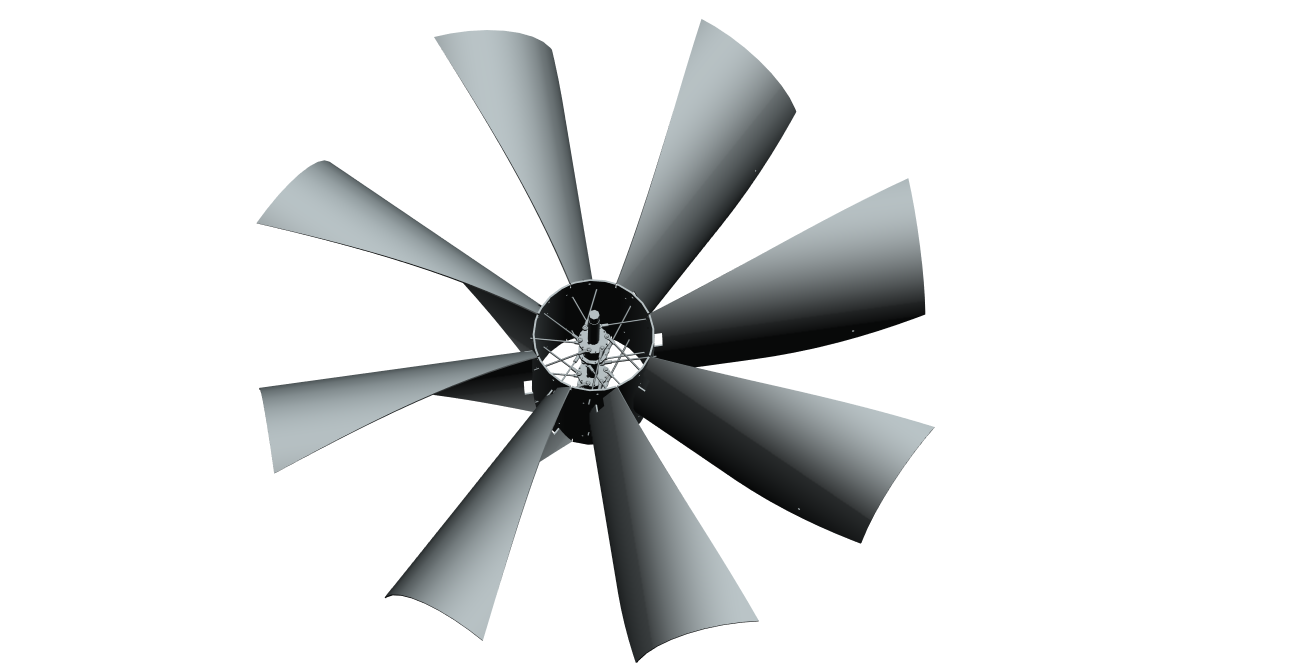
\includegraphics[width=.53\linewidth]{rotor_assem_oblique_2}
    \end{figure}

    \begin{figure}[htb]
     \centering
     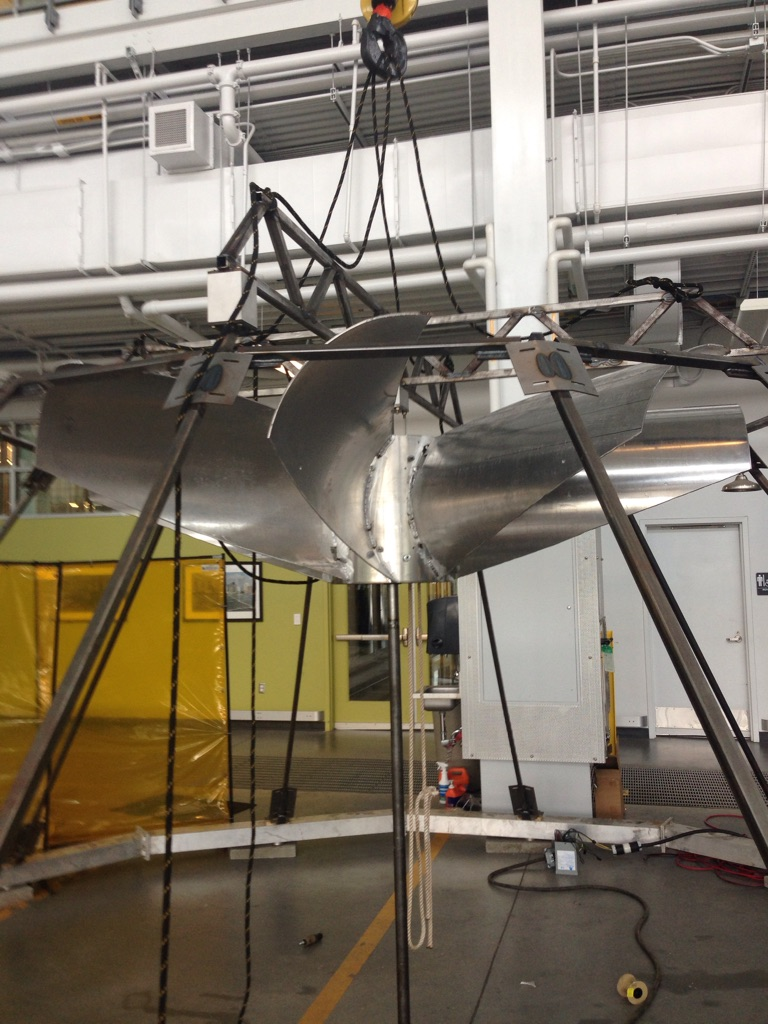
\includegraphics[width=.2\linewidth]{turbine_built}
    \end{figure}

 turbine energy?

 turbine placed at top of vanes

 gap in turbine 

\end{frame}



%
%
\begin{frame}
 \frametitle{Solution Structure}


\begin{figure}[!htb]
  \centering
  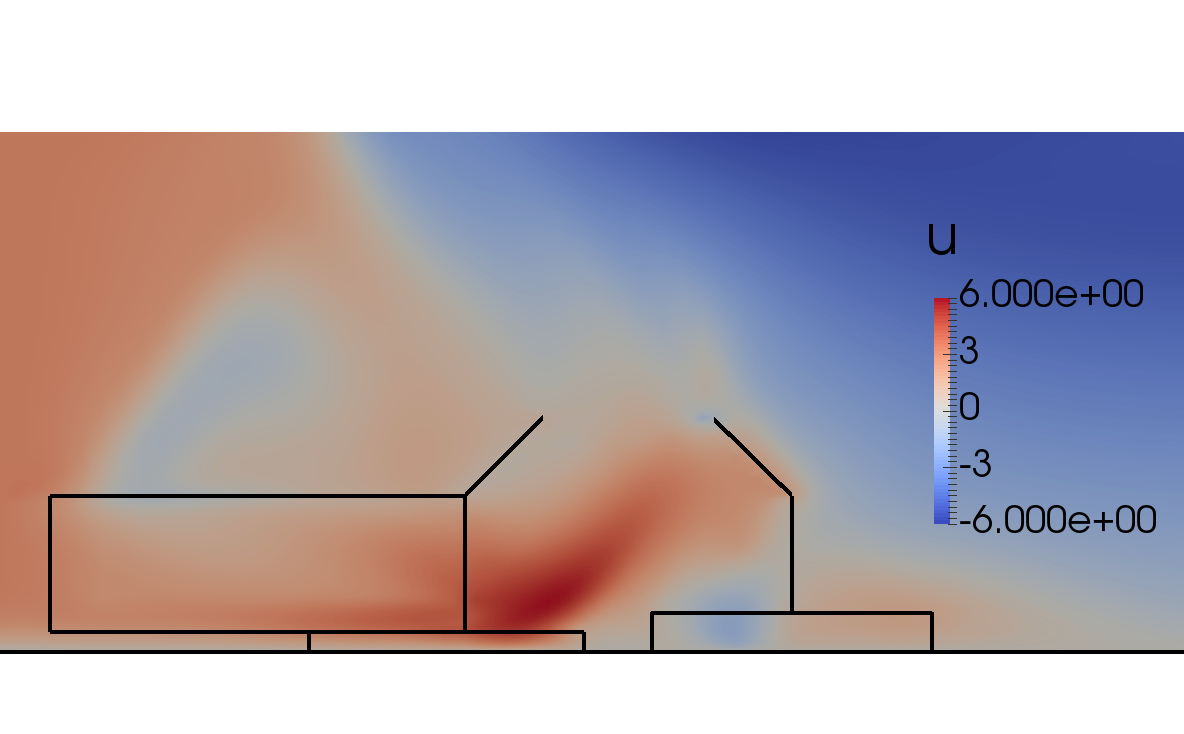
\includegraphics[width=.47\linewidth]{u_field_vert}
  \hfill
  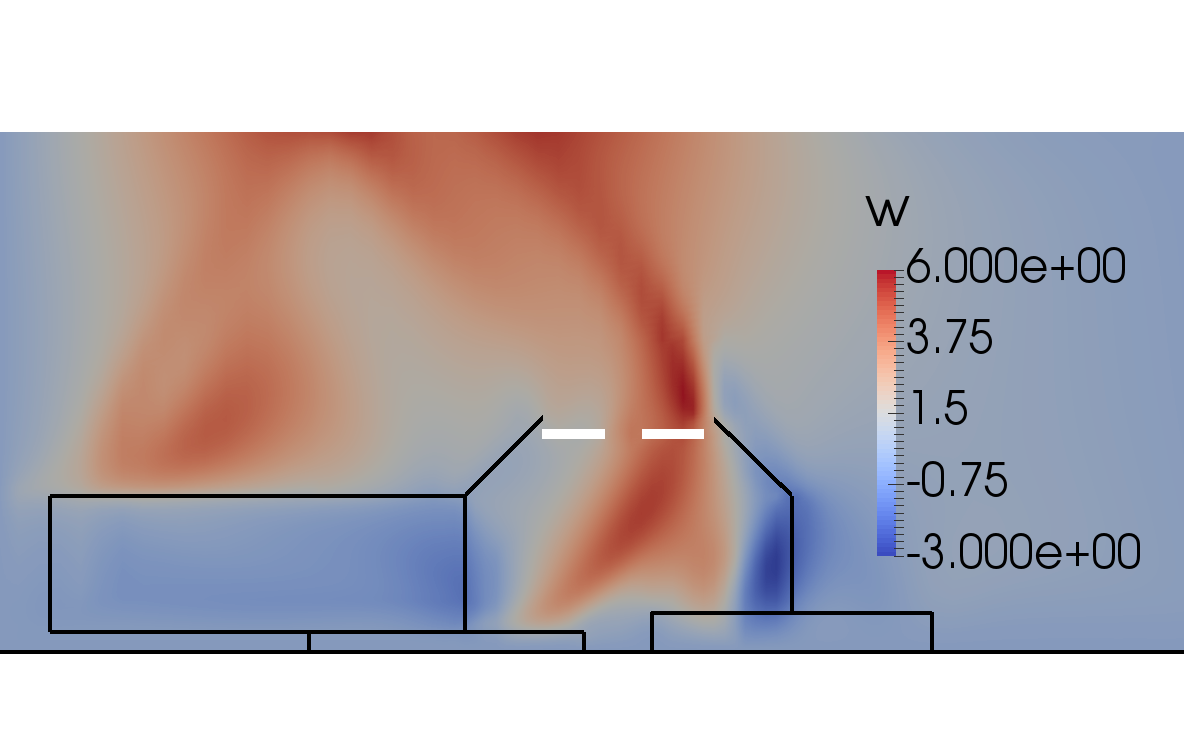
\includegraphics[width=.47\linewidth]{w_field_vert}
  \\
  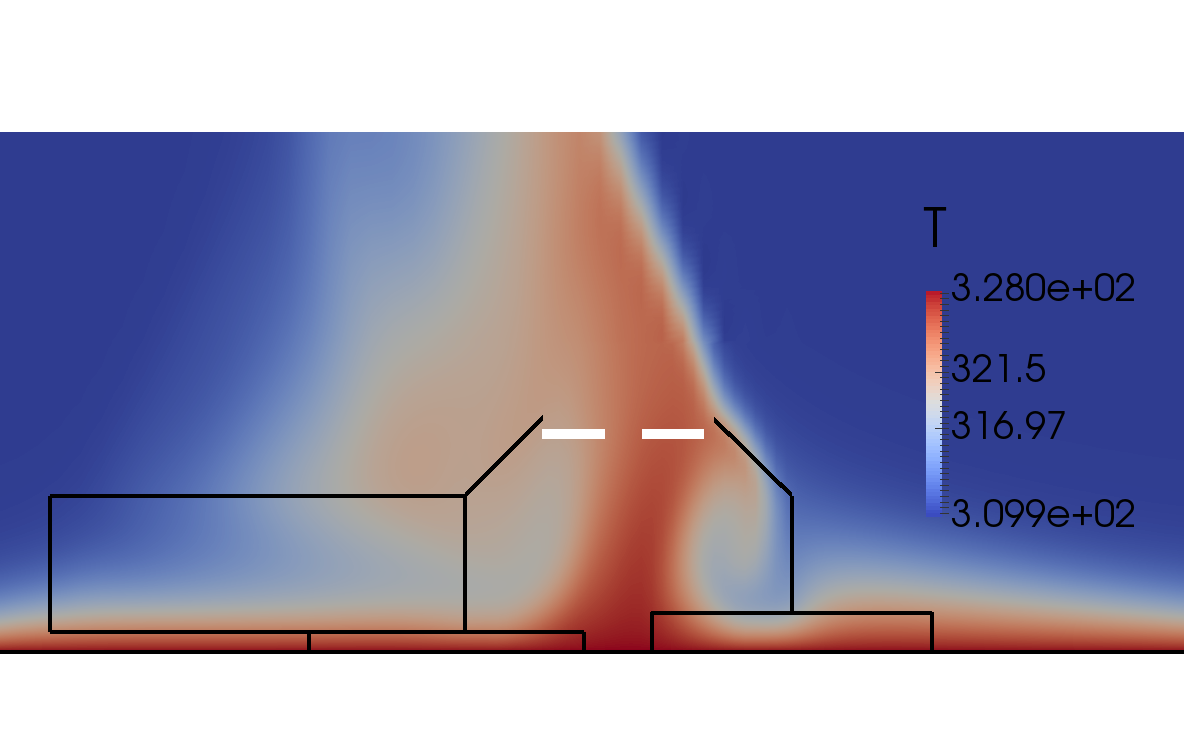
\includegraphics[width=.47\linewidth]{T_field_vert}
  \hfill
  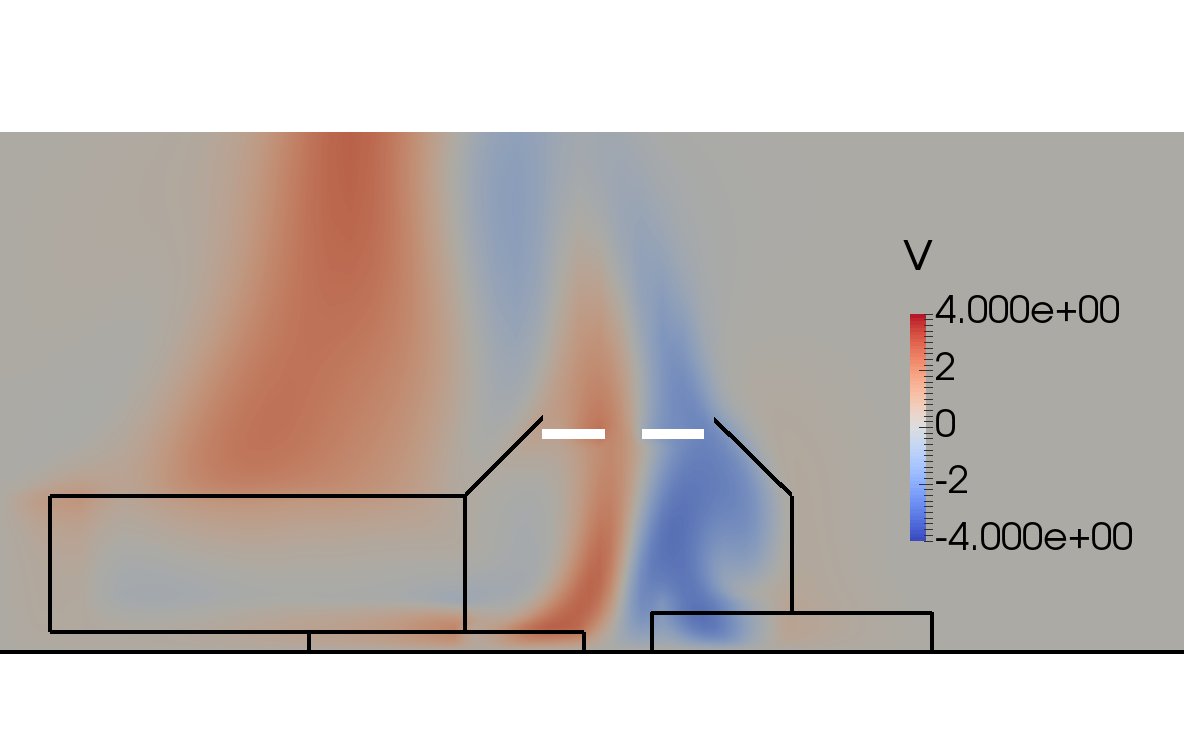
\includegraphics[width=.47\linewidth]{v_field_vert}
\end{figure}

\end{frame}

%
%
%
\begin{frame}
 \frametitle{Solution Structure}


\begin{figure}[!htb]
  \centering
  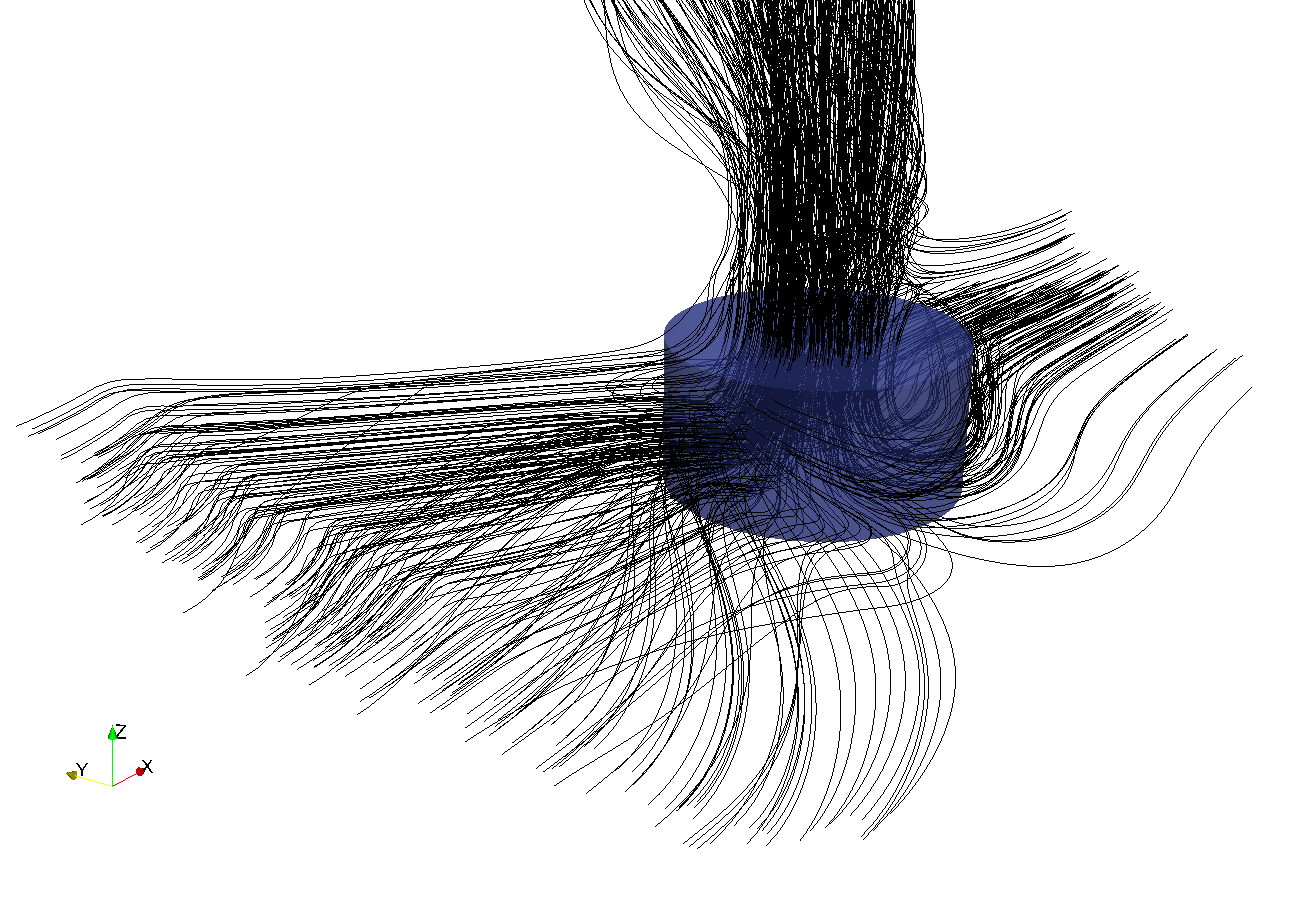
\includegraphics[width=.67\linewidth]{field_streamlines}
 \end{figure}

\begin{block}{title}
 \begin{itemize}
  \item Entraining fluid from wide region in front of device
  \item Substantial portion of backflow also included
\end{itemize}
\end{block}

\end{frame}


%
%
%
\begin{frame}
 \frametitle{2016 Field Test}

\begin{block}{What we know}
\begin{itemize}
 \item Little or no flow through device
 \item Configuration largely consistent with CFD
\end{itemize}
\end{block}

\begin{block}{Possible problems}
\begin{itemize}
 \item Shading
       \begin{itemize}
	\item ground temperature inside the vane region set to the ambient air 
       \end{itemize}
 \item Closed back vanes
       \begin{itemize}
	\item reduced but non-zero power
       \end{itemize}
 \item Poor field conditions
       \begin{itemize}
	\item Poor field conditions (intermittent winds, $100^{\circ}$
	      F, etc.)  
       \end{itemize}
\end{itemize}
\end{block}

\bigbreak
\centering 
Several other possible model corrections were investigated

\end{frame}

%
%
%
\begin{frame}
 \frametitle{Drag addition}
\begin{itemize}
 \item Initial analysis indicated drag not significant
 \item Revisited after 2016 Field test
 \item Model introduced skin-friction effects
 \item Drag computed based on smallest distance between vanes
       \begin{itemize}
	\item ``worst-case'' scenario
       \end{itemize}
 \item Kinetic energy flux never reduced by more than 12\%.
\end{itemize}


\end{frame}


\begin{frame}
\frametitle{Drag Addition}

\end{frame}

%
%
\begin{frame}
 \frametitle{Solidity Modification}

\end{frame}

%
%
\begin{frame}
 \frametitle{Solidity Modification}


 \begin{columns}[]
  \begin{column}{0.55\linewidth}


   \begin{center}
    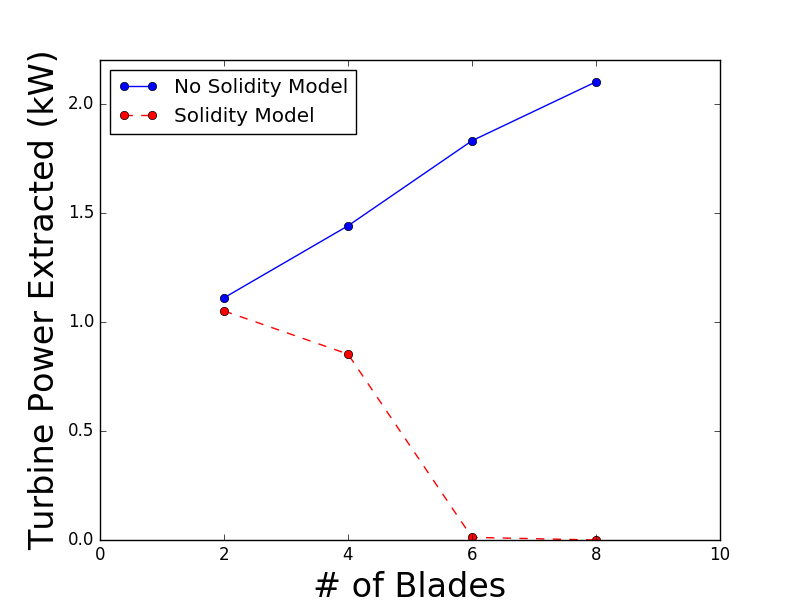
\includegraphics[width=1.1\linewidth]{solidity}
   \end{center}

  \end{column}
  \begin{column}{0.45\linewidth}
   
   \begin{block}{Correction to actuator disk}
    \begin{itemize}
     \item Model assumes flow separates from turbine blade
	   \begin{itemize}
	    \item ``worst case'' estimate
	   \end{itemize}
     \item Six and eight turbine blades greatly impacted
     \item Need calibration/validation data for more detailed assessment  
	   \begin{itemize}
	    \item Data needed from field or gridded simulation
	   \end{itemize}
     \item Even with correction, model appears inadequate
    \end{itemize}

   \end{block}
  \end{column}
 \end{columns}

\end{frame}



%
%
\begin{frame}
 \frametitle{Idealized Turbine Drag Polars}

in contrast to previous efforts, 
we now optimize power extraction for a generic turbine

\end{frame}


%
%
\section{Conclusions}
\begin{frame}
 \frametitle{System Feasibility Assessment}

 \begin{block}{Not competitive with Photovoltaics}
 \begin{itemize}
 \item Assume 1000~W/$\text{m}^2$, efficiency of 15\%
 \item Order of magnitude less power for same 6 meter diameter
 \end{itemize}
 \end{block}


 \begin{block}{Additional Risks}
 \begin{itemize}
 \item No validation
 \item Solutions are ``Fragile''
 \end{itemize}
 \end{block}

 \begin{block}{Additional Notes}
 \begin{itemize}
 \item Independent of economic assessment (e.g. $kW/\$$?)
 \item Why is power generated by SoV lower than Natural?
 \end{itemize}
 \end{block}


\end{frame}

%
%
\begin{frame}
 \frametitle{Conclusions and Future Work}
 
 \begin{block}{Contributions}
  \begin{itemize}
   \item Turbine Solidity Implications for Actuator Disk?
  \end{itemize}
 \end{block}


\end{frame}

%
%
%
 \begin{frame}
   \frametitle{The End}

   \begin{figure}[htb]
     \centering
     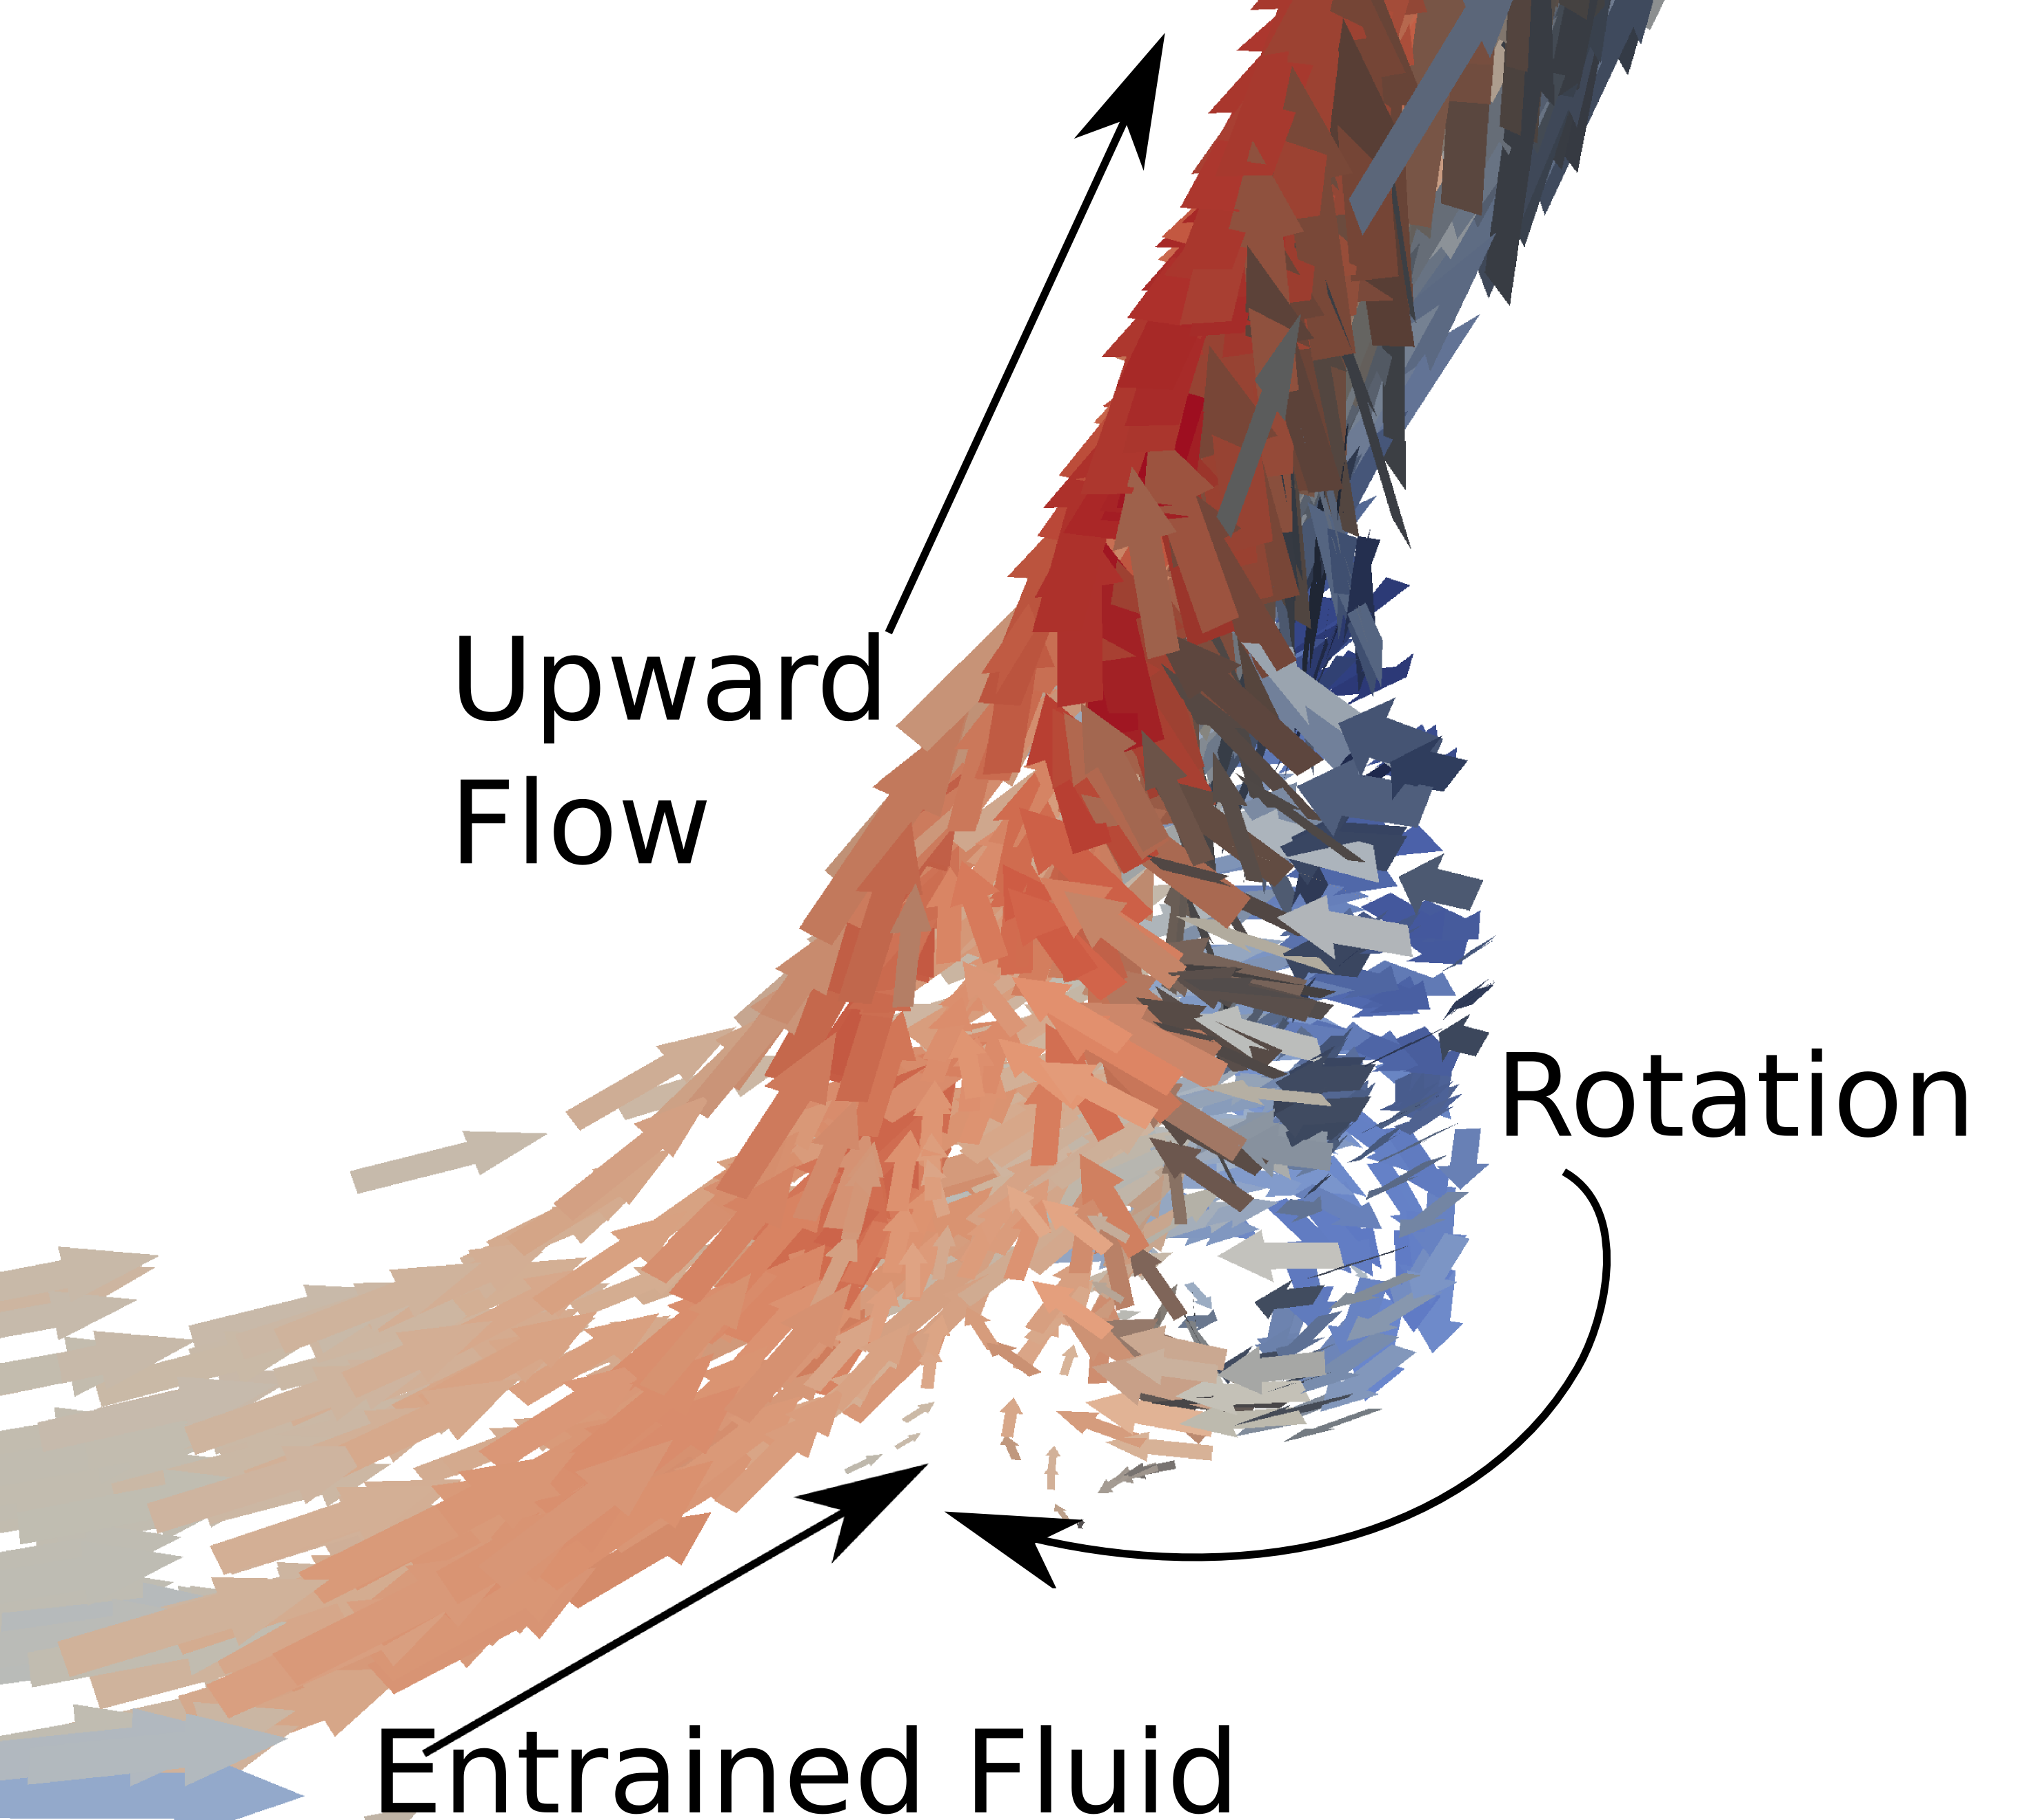
\includegraphics[width=.55\linewidth]{arrows}
   \end{figure}

   \begin{block}{Thank you!}
    \center{nick@ices.utexas.edu}
    \end{block}
 \end{frame}


%%%%%%%%%%%%%%%%%%%%%%%%%%%%%%%%%%%%%%%%%%%%%%%%%%%%%%%%%%%%%%%%%%%%%%%%%%%%%%
% BONUS ROUND
%%%%%%%%%%%%%%%%%%%%%%%%%%%%%%%%%%%%%%%%%%%%%%%%%%%%%%%%%%%%%%%%%%%%%%%%%%%%%%
%
\appendix
\section{Extra Slides}

%
% scaling
%
\begin{frame}
  \frametitle{Estimate of Energy Scaling}
    \begin{itemize}
    \item Medium size dust devil: $3\text{m} = \text{D}$, $U =  5 \text{
	  m/s}$, $\Delta T = 30$ K, $3$ meters tall
    \item Assume a turbulent boundary layer ($\delta = 10$ cm),
      \begin{equation*}
        u(z) = U \text{ min }\left(\left(\frac{z}{\delta}\right)^7,1\right)
      \end{equation*}        
    \end{itemize}

  \begin{columns}[]
    \begin{column}{0.45\linewidth}
      Boussinesq potential energy flux over the upstream flow [Renno]:
      \begin{align*}
        E_p & = \int u(z) (\rho(z)-\rho_\infty) g z \, dA \\
        E_p & = g  \pi R \beta \rho_0 U \Delta T \left[ \frac{z_\text{max}^2}{2} - \frac{7 \delta^2}{18} \right] \\
       & = 217 \text{ Watts}
      \end{align*}

    \end{column}
  %
    \begin{column}{0.55\linewidth}
      The KE flux:  surface integral over upstream face of dust devil: 
      \begin{align*}
        \text{KE} & = \int \frac{\vec V^2}{2} \rho \vec V \cdot \hat n \, dA \\
        \text{KE} & = R \rho U^3 \left[ z_{\text{max}} - \frac{10}{11}\delta \right] \\
        & = 1144 \text{ Watts}
      \end{align*}
    \end{column}
  \end{columns}
\end{frame}


%
%
%
\begin{frame}
\frametitle{Calibration of Virtual Vanes}

    \begin{figure}[htb]
     \centering
     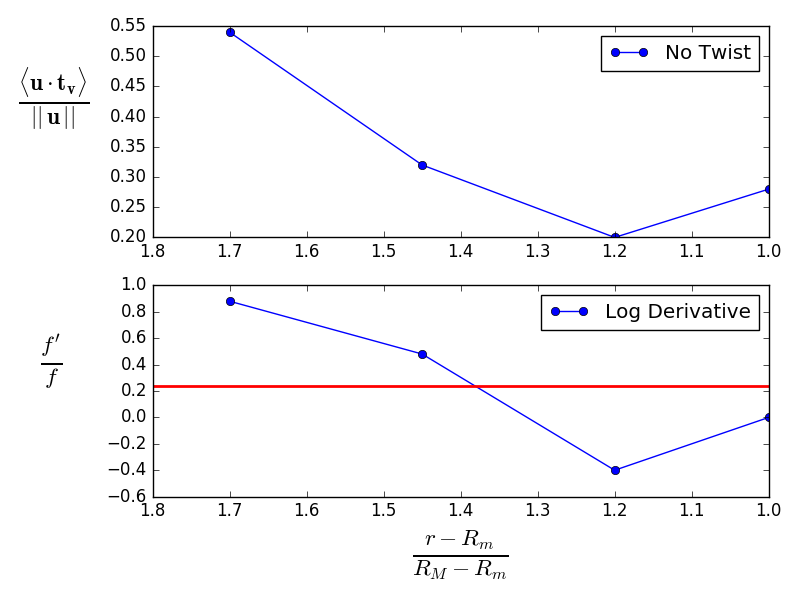
\includegraphics[width=.85\linewidth]{annealing}
    \end{figure}
\end{frame}

%
% mesh
%
\begin{frame}
 \frametitle{Mesh}
 
 \begin{figure}[htb]
  \centering
  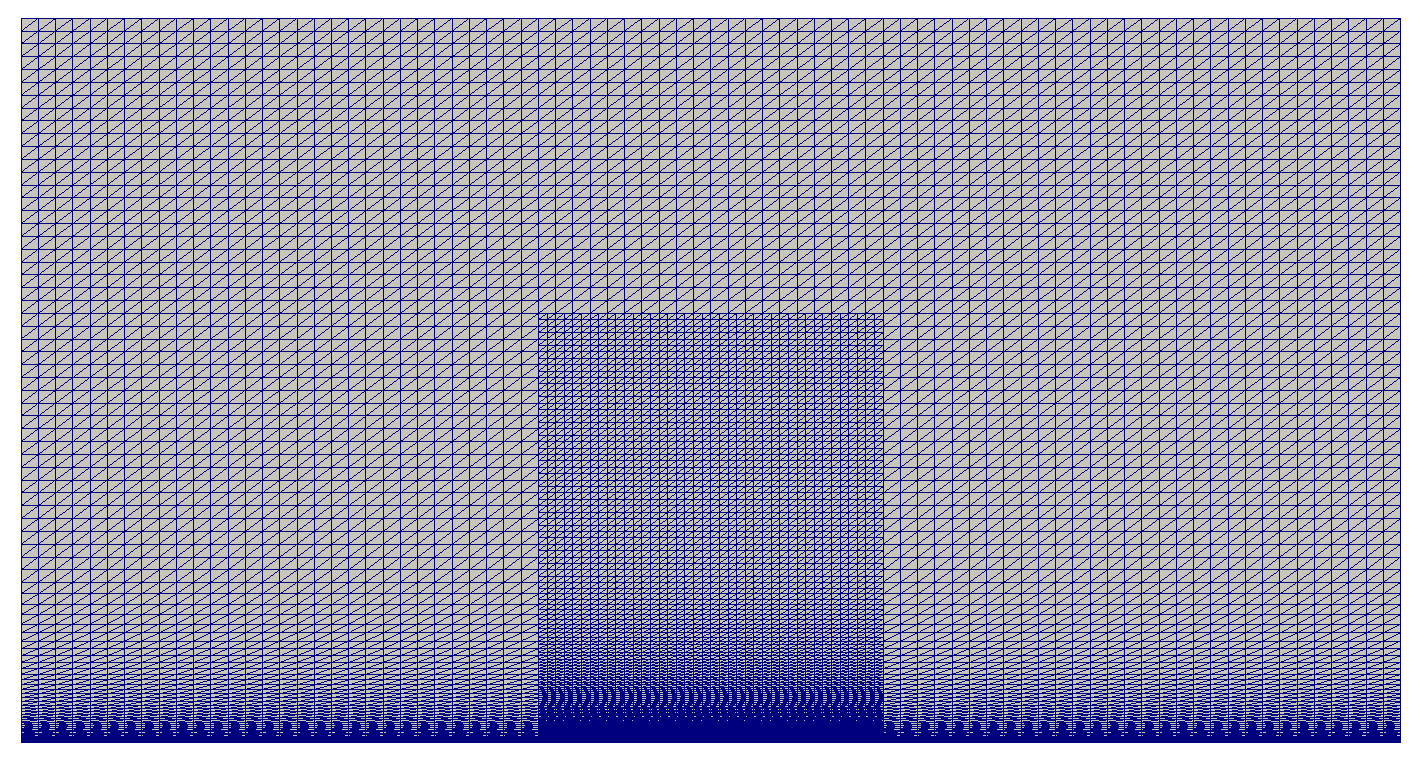
\includegraphics[width=.55\linewidth]{meshing}
 \end{figure}
 
 \begin{block}{Discretization}
  \begin{itemize}
   \item Single refinement in vane region
  \end{itemize}
\begin{equation*}
	  \text{Re}_\text{cell} = \frac{\text{max}(\Delta x,\Delta y)
	   \, u}{\nu_T}
\end{equation*}	
  \begin{itemize}
   \item Boundary layer mesh visible
  \end{itemize}
 \end{block}
\end{frame}

%
% SUPG Stab
%
\begin{frame}
\frametitle{Stabilization Outline}

\begin{itemize}
 \item Cast Navier Stokes + Boussinesq equations into weak form
 \item Prepare as operator $Lc=f$
 \item Calculate Fr\'echet derivative (to calculate operator adjoint)
 \item Separate into differential (P) and constant (Z) components,
       $L'[c] = P + Z$
 \item Choose stabilization operator such that $S = -P^*$
 \item Then stabilization has form, $a_h(c,\phi) = a(c,\phi) + \langle
       Lc,S\phi \rangle_\tau$
\end{itemize}
\end{frame}

%
%
%
\begin{frame}
\frametitle{Simulation Geometry and Boundary Conditions}

\begin{block}{Specified Inflow}

   \begin{itemize}
   \item 7th order turbulent boundary layer, 
     \begin{equation*}
       u_{\text{in}}(z) = U \text{ min }\left(\left(\frac{z}{\delta}\right)^7,1\right)
       \label{eq:bl_u}
     \end{equation*}
   \item The thermal inflow is then,
     \begin{equation*}
       T_{\text{in}}(z) = \Delta T \left(1- \text{ min
       }\left(\left(\frac{z}{\delta}\right)^7,1\right)\right)
       + T_0 \textcolor{blue}{- \beta}.  
     \end{equation*}
   \end{itemize}
\end{block}

\begin{block}{Ground}
  \begin{itemize}
    \item modeled with a Dirichlet boundary condition such that, 
      \begin{align*}
        {\bf u} &= 0 \quad \text{ on } \Gamma_G \\
        T &= T_g
      \end{align*}
  \end{itemize}
  \end{block}

\end{frame}

%
%
%
\begin{frame}
\frametitle{Field Validation Study}
 
\begin{columns}[]
  \begin{column}{0.52\linewidth}
   \begin{block}{Scenario parameter uncertainty}
    \begin{itemize}
     \item Wind speed: 2-5 m/s
     \item Wind direction($\approx20^{\circ}$)
     \item $T_{\text{s}} = 50-60^{\circ}$ C ($\approx 121-140^{\circ}$ F)
     \item No boundary layer temperature data 
	   (DAQ equipment malfunctioned)
    \end{itemize}
   \end{block}
  \end{column}

  \begin{column}{0.49\linewidth}

   \begin{center}
    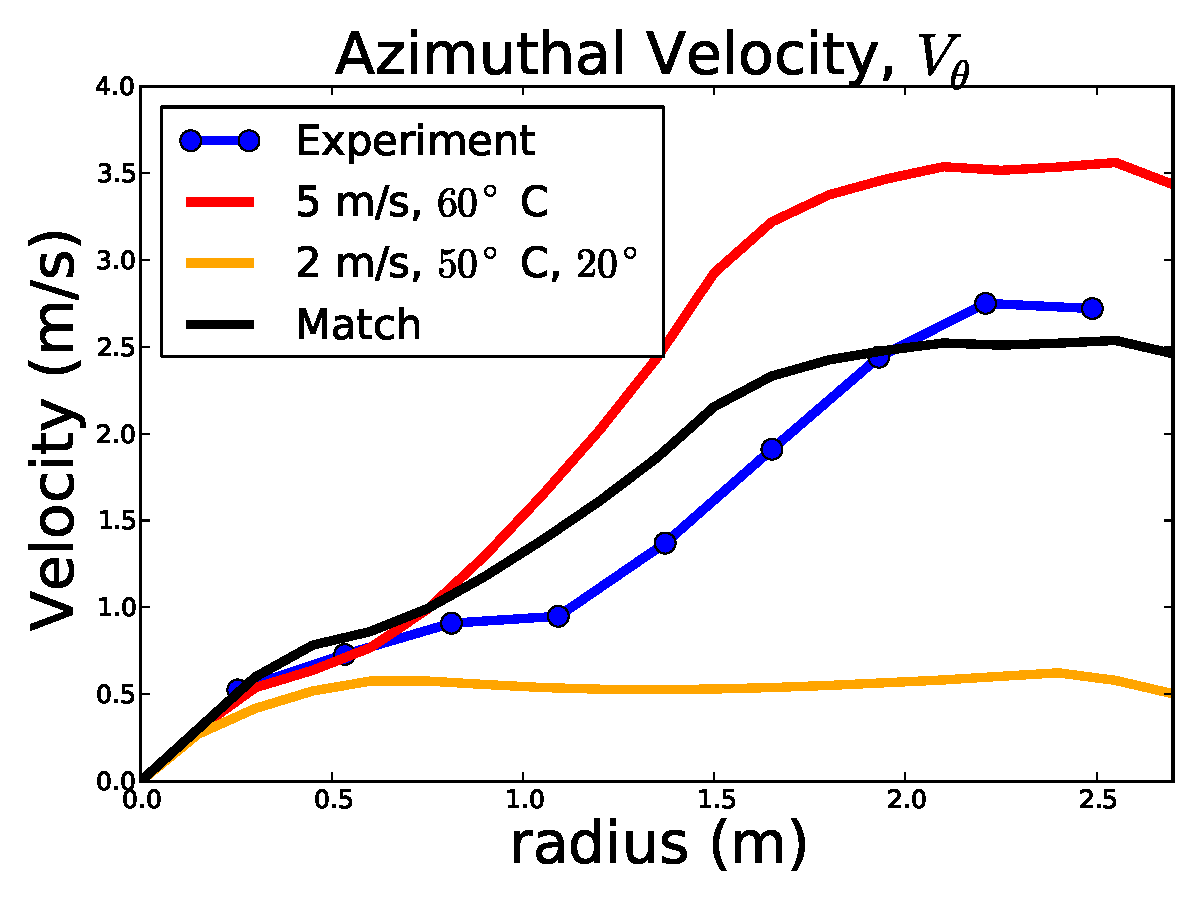
\includegraphics[width=0.99\linewidth]{validate_field}
   \end{center}
  \end{column}
 \end{columns}

 \begin{center}
  \begin{itemize}
   \item CFD broadly consistent with field observations
	 \begin{itemize}
	  \item Experimental data extremely limited
	 \end{itemize}
   \item Kinetic energy fluxes match to within 10\%
  \end{itemize}
  \end{center}

\end{frame}


%
%
%
\begin{frame}
\frametitle{Thermal-Only Structure}

\begin{figure}[!htb]
  \centering
  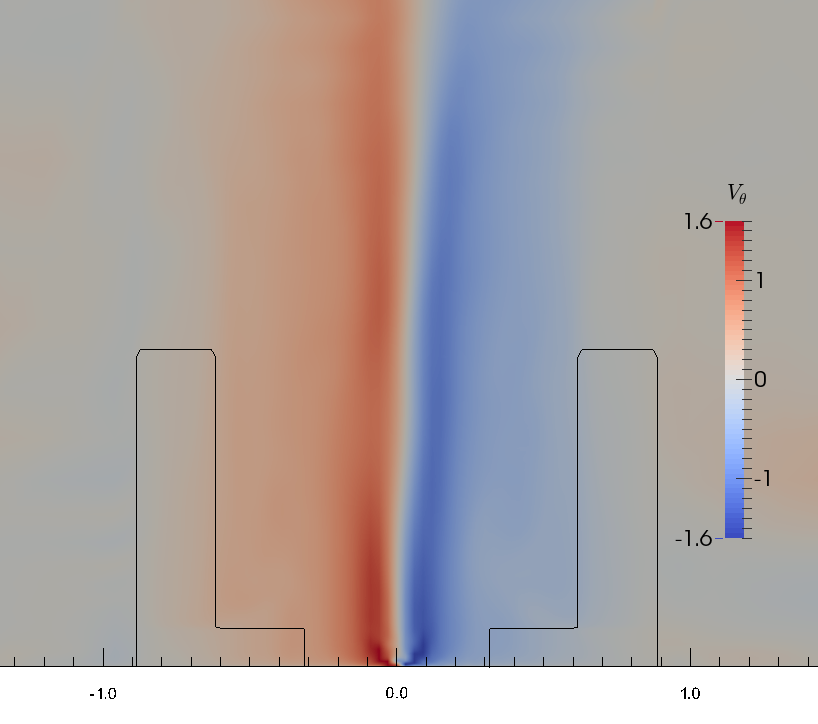
\includegraphics[width=.38\linewidth]{vt}
  \hfill
  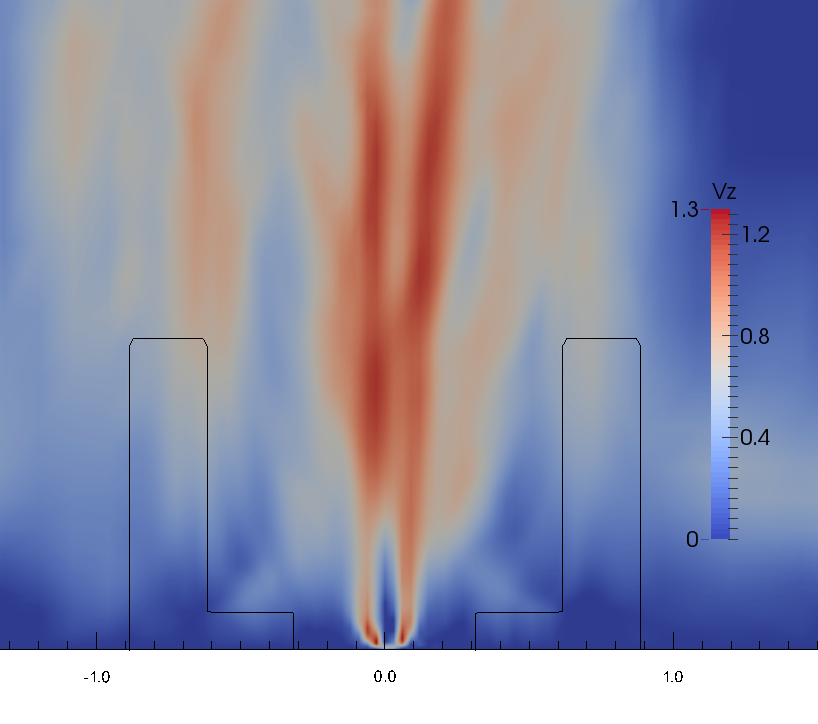
\includegraphics[width=.38\linewidth]{vz}
  \\
  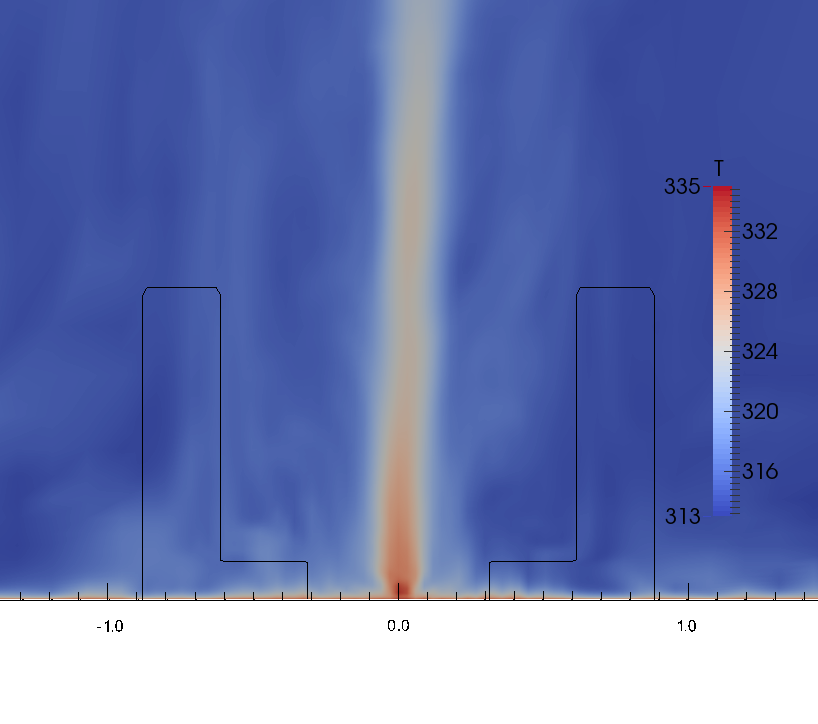
\includegraphics[width=.38\linewidth]{t}
  \hfill
  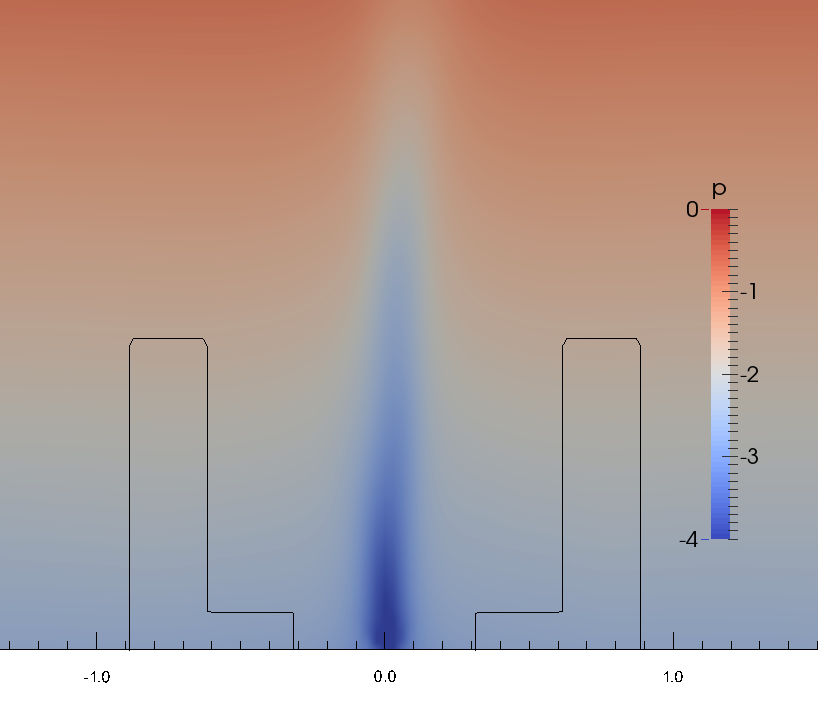
\includegraphics[width=.38\linewidth]{p}
\end{figure}


\end{frame}

%
%
%
\begin{frame}
\frametitle{Thermal-Only Structure}

    \begin{figure}[htb]
     \centering
     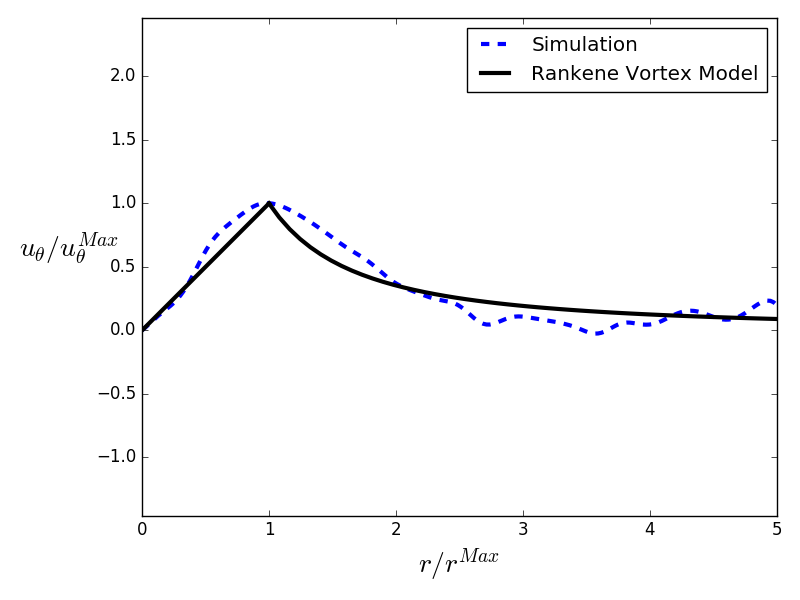
\includegraphics[width=.85\linewidth]{rankene}
    \end{figure}
\end{frame}

%
%
%
\begin{frame}
\frametitle{Proposal Timeline}
\small
\begin{center}
\begin{table}
\centering
\begin{minipage}[t]{1.6\linewidth}
\color{black}
 \rule{\linewidth}{1pt}
 \yto{April 2016}{Conclude parameter sweeps and optimization of apparatus}
 \yto{April 2016}{Turbine actuator-disk verification, validation and prediction}
 \ytl{May 2016}{Proposed configuration and predictions for experimental
 team}
 \ytb{July 2016}{Comparisons between synthetic and natural dust devil physics}
 \ytl{Aug 2016}{Validation against 2016 field data}
 \ytl{Sept 2016}{Optimal drag polar prediction}
\ytl{Nov. 2016}{Dissertation Defense}
 \bigskip
 \rule{\linewidth}{1pt}%
\end{minipage}%
\end{table}
 \label{tab:prop}
\end{center}

\end{frame}


%
%
%
\begin{frame}
 \frametitle{Course list}
 \footnotesize
 \begin{table}[h]
  \centering
  \begin{tabular}{llll}
   \hline \hline
   Course \# & Semester & Course Name & Instructor \\ 
   \hline 
   ME381P   & 2014 Spr.   & Validation \& Uncertainty Quantification &
	       Prof. R.D. Moser \\
   ME 382R5 & 2014 Spr.   & Advanced Combustion & Prof. O.A. Ezekoye \\
   CSE 397  & 2014 Spr.   &  Comp. \& Var. Methods for
	   Inv. Problems & Prof. O. Ghattas \\
   SDS 384  & 2014 Fall   & Bayesian Statistical Methods & Prof. S.
	       Walker \\
   SDS 394  & 2014 Fall   & Scientific \& Technical Computing & Dr. V. Eijkhou \\
   ME 382P  & 2015 Fall   & Adv. Exp. Methods in Thermal/Fluids
	   & Prof. D. Bogard \\  
   \hline \hline
  \end{tabular} 
 \end{table}

\end{frame}


\end{document}
